\chapter{Grundlagen}

Dieses Kapitel dient als umfassende Grundlage für die Erforschung der Rolle neuronaler Netze in der Optimierung und Steuerung von PID-regulierten DC-Konvertern. Im Fokus stehen sowohl die Grundlagen der DC-DC-Konvertertechnologie als auch spezielle Herausforderungen, die in diesem Kontext auftreten können, wie beispielsweise die altersbedingte Degradation von Schaltungskomponenten. Darüber hinaus bietet das Kapitel einen Überblick über moderne Optimierungsmethoden wie DDPG (Deep Deterministic Policy Gradients) . Der Inhalt dieses Kapitels zielt darauf ab, den Leser umfassend auf die Herausforderungen, technischen Lösungen und innovativen Ansätze in diesem sich schnell entwickelnden Forschungsfeld vorzubereiten.

%1. Gleichspannungswandler (DC-DC-Konverter)


\section{Elektrotechnik}
\subsection{Buck-Konverters}
\label{sec:DCDC_Konverter}

\paragraph{Hauptkomponenten und Funktionen eines DC-DC-Konverters}

Die Wandlung von Gleichspannung (DC) in eine andere Gleichspannung ist ein kritischer Aspekt in der Elektronik und Energieversorgung. Ein weit verbreitetes Schaltungsdesign, das diese Funktion ausführt, ist der Buck-Konverter. In der Literatur wird dieser als eine Standardmethode für DC-DC-Wandlung beschrieben \cite{wensdesign2022}.



\paragraph{MOSFET-Transistor}
Der MOSFET-Transistor agiert als elektronischer Schalter, der den Stromfluss in der Schaltung reguliert. Gegenüber Bipolartransistoren, einer traditionellen Wahl für Schaltaufgaben, bietet der MOSFET eine signifikante Effizienzsteigerung durch seine minimalen Leistungsverluste. Dieser Vorteil resultiert aus inhärenten physikalischen Eigenschaften wie der hohen Trägermobilität, die zu einem geringeren Durchlasswiderstand führen und somit eine robuste Widerstandsfähigkeit gegenüber thermischen Ausfällen gewährleisten. \cite{choi2013pulsewidth}.

\paragraph{Induktivität (Spule)}
Die Induktivität dient der temporären Energiespeicherung in Form eines magnetischen Feldes, das beim Stromfluss durch die Spule generiert wird. Dies ist insbesondere relevant in Anwendungen wie Solenoid-Antriebsschaltungen, wo die Induktivität als Energiespeicher und -überträger fungiert \cite{choi2013pulsewidth}.

\paragraph{Diode}
Die Diode ist so ausgerichtet, dass sie den Strom nur in einer Richtung passieren lässt. Dies ist insbesondere wichtig, wenn der MOSFET-Transistor deaktiviert ist. Als passive Schalter werden oftmals schnelle Erholungsdioden oder Schottky-Dioden aufgrund ihrer exzellenten Schalteigenschaften verwendet \cite{choi2013pulsewidth}.

\paragraph{Kondensator}
Der Kondensator dient der Glättung der Ausgangsspannung und speichert Energie für die Last. Er spielt eine wichtige Rolle in der Dynamik der Schaltung und ermöglicht eine stabilere Energieversorgung \cite{Kularatna2012}.
\paragraph{Regelung und Anwendungen}

In der Praxis werden Buck-Konverter oft von einer nicht-idealen Spannungsquelle gespeist und müssen daher unter variablen Eingangsspannungen und Lastströmen arbeiten \cite{choi2013pulsewidth}. Daher ist eine geschlossene Regelungsschleife erforderlich, um eine konstante Ausgangsspannung sicherzustellen.

Buck-Konverter finden eine breite Anwendung in verschiedenen elektronischen Geräten und Systemen. Ihr hoher Wirkungsgrad, der in der Regel zwischen 75\% und 98\% liegt, macht sie besonders attraktiv.


\begin{figure}[htbp]
    \centering
    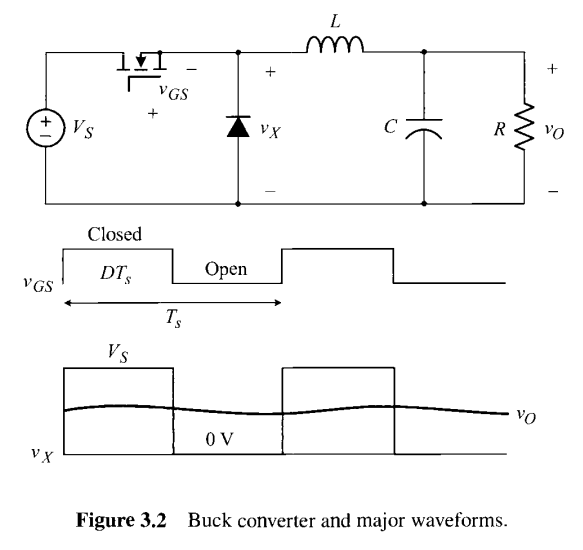
\includegraphics[width=0.4\linewidth]{2Grundlagen/111DCDC.png}
    \caption{Schematische Darstellung eines DC-DC Konverters. Quelle: \cite{choi2013pulsewidth}}
    \label{fig:dcdc_converter}
\end{figure}




\subsection{Degradation von Kondensatoren und MOSFETs in DC-DC-Konvertern}

Die Zuverlässigkeit und Effizienz von DC-DC-Konvertern sind zunehmend von der Degradation ihrer Schlüsselkomponenten, insbesondere von Kondensatoren und MOSFETs, beeinträchtigt.

\paragraph{Kondensatoren}

Kondensatoren sind anfällig für verschiedene Arten von Ausfallmodi, darunter Änderungen des Verlustfaktors (tan $\delta$), der Impedanz und des Dissipationsfaktors. Diese Parameter sind entscheidend für die Beurteilung der Zuverlässigkeit eines Systems. Ebenso ist die erhöhte Äquivalente Serienresistenz (ESR) von Elektrolytkondensatoren, die elektrischen und thermischen Belastungen ausgesetzt sind, ein weiterer entscheidender Faktor für die Degradation.\cite{jeong2023degradation}

\paragraph{MOSFETs}

Bei MOSFETs kann die Degradation aufgrund von thermischen Spannungen zu einem Gate-Source-Kurzschluss oder einem Drain-Source-Kurzschluss führen. Die Degradation der Transistoren erhöht deren Leistungsverluste und beschleunigt damit den Degradationsprozess weiter.\cite{wensdesign2022}



\paragraph{Kontrolle und Überwachung}

Aktuelle Forschungsbemühungen konzentrieren sich auf die Entwicklung von Kontrollalgorithmen, um die Degradation zu verzögern und die Zuverlässigkeit der Konverter zu erhöhen. Dazu gehören auch Verfahren zur Schätzung des Zustands der Degradation in Echtzeit.
\cite{choi2013pulsewidth}

\paragraph{Integration mit neuronalen Netzen für Kondensatoren und MOSFETs}

Neuronale Netze können verwendet werden, um aktiv entgegensteuernde Maßnahmen zur Verlangsamung der Degradation von Schlüsselkomponenten wie Kondensatoren und MOSFETs in DC-DC-Konvertern einzuleiten. Durch die kontinuierliche Analyse von Betriebsparametern wie Temperatur und Spannung sind diese Netze in der Lage, den Zustand der Degradation in Echtzeit zu erfassen. Sobald kritische Zustände, die auf Degradation hindeuten, erkannt werden, können die neuronalen Netze automatisch die PID-Koeffizienten des Konverters anpassen. Dies dient dazu, die Auswirkungen der Degradation zu minimieren und die Zuverlässigkeit des Systems zu erhöhen.
\cite{morales2020grokking}

\subsection{PID-Regler}
\label{sec:PID-Regler}

Der PID-Regler ist eine essenzielle Komponente in der Automatisierungstechnik und wird zur Regelung verschiedener Prozessgrößen wie Geschwindigkeit, Temperatur und Spannung eingesetzt.

\paragraph{Proportionalanteil (P)} \mbox{}\\
Der Proportionalanteil reagiert direkt auf den aktuellen Fehlerwert \( e(t) \), indem er diesen mit der Proportionalverstärkung \( K_p \) multipliziert:
\begin{equation}
P_{\text{out}} = K_p \cdot e(t)
\end{equation}

\paragraph{Integralanteil (I)} \mbox{}\\
Der Integralanteil akkumuliert kontinuierlich die Fehlerwerte und multipliziert das Ergebnis mit der Integralverstärkung \( K_i \), um den kumulierten Fehler zu korrigieren:
\begin{equation}
I_{\text{out}} = K_i \cdot \int e(t) \, dt
\end{equation}

\paragraph{Differentialanteil (D)} \mbox{}\\
Der Differentialanteil betrachtet die Änderungsrate des Fehlers und multipliziert sie mit der Differentialverstärkung \( K_d \):
\begin{equation}
D_{\text{out}} = K_d \cdot \frac{d}{dt} e(t)
\end{equation}

\paragraph{PID-Regelungsgleichung} \mbox{}\\
Diese drei Anteile kombiniert ergeben den gesamten Steuerausgang des PID-Reglers:
\begin{equation}
\text{Steuerausgang} = P_{\text{out}} + I_{\text{out}} + D_{\text{out}}
\end{equation}

\paragraph{Einstellung der Verstärkungsfaktoren} \mbox{}\\
Die sorgfältige Einstellung der Verstärkungsfaktoren \( K_p, K_i, \) und \( K_d \) ist entscheidend, um eine optimale Systemleistung zu erzielen.

\paragraph{Anwendung bei Gleichstrom-Gleichstrom-Wandlern} \mbox{}\\
PID-Regler werden verwendet, um die Ausgangsspannung von DC-DC-Wandlern zu stabilisieren, indem sie ständig die Ist-Spannung mit der Soll-Spannung vergleichen und entsprechend regulieren.
\cite{SwainBaid2014}

\paragraph{Fazit} \mbox{}\\
Der PID-Regler ist aufgrund seiner Effizienz und Anpassungsfähigkeit für eine Vielzahl von Anwendungen geeignet.

\begin{figure}[htbp]
    \centering
    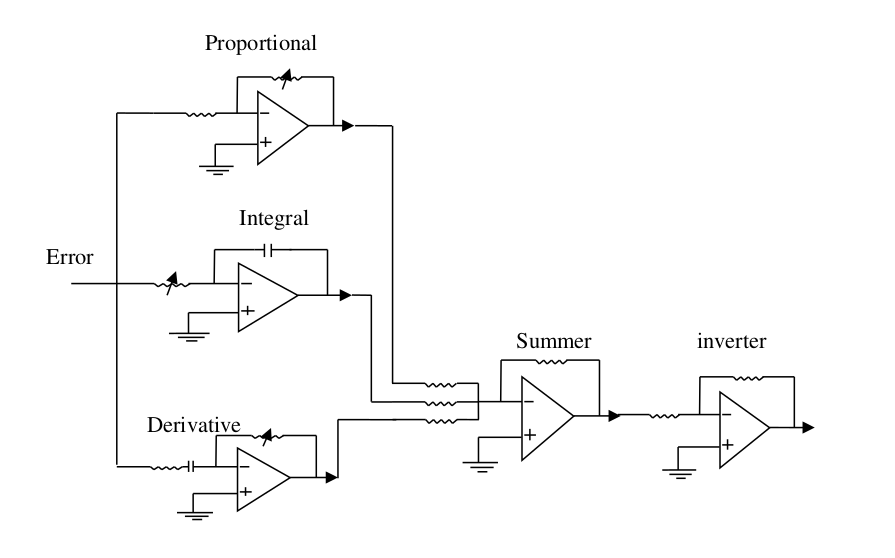
\includegraphics[width=0.6\linewidth]{2Grundlagen/13PID.png}
    \caption{Schematische Darstellung eines PID-Regler. Quelle: \cite{SwainBaid2014}}
    \label{fig:PID_converter}
\end{figure}

\paragraph{Zusammenfassung der PID-Reglerkomponenten} \mbox{}\\
Der PID-Regler passt das Systemverhalten durch die proportionale, integrale und differenzielle Reaktion auf Fehlerwerte an. Die Zusammenarbeit dieser drei Komponenten sorgt für ein ausgewogenes und effektives Regelungssignal.





\subsection{Pulsweitenmodulation und ihre Darstellung}
\label{sec:PWM_Grundlagen}
Pulsweitenmodulation (PWM) ist eine Schlüsseltechnik in DC-DC-Wandlern, die zur Steuerung der Schaltkomponenten eingesetzt wird, um die Ausgangsspannung oder den Ausgangsstrom zu regulieren. Sie ermöglicht eine präzise Kontrolle, indem sie die 'Einschaltzeit' des Schalters im Vergleich zur gesamten Zykluszeit (Einschaltzeit + Ausschaltzeit) variiert.\cite{peddapelli2017pulse}

\paragraph{Tastverhältnis \(D\)}
Die Einschaltzeit ist die Zeit, der Schalter eingeschaltet ist. Das Tastverhältnis \( D \) wird mathematisch als das Verhältnis der Einschaltzeit zur gesamten Zykluszeit beschrieben:
\begin{equation}
D = \frac{\text{Einschaltzeit}}{\text{Einschaltzeit} + \text{Ausschaltzeit}}
\end{equation}

\paragraph{Proportionalanteil (P)}
Das Tastverhältnis spielt eine wichtige Rolle, da es den Mittelwert der Ausgangsspannung oder des Ausgangsstroms bestimmt. Bei der PWM wird ein Steuersignal mit einem hochfrequenten Trägersignal verglichen, um die 'Ein'- und 'Aus'-Zustände des Schalters festzulegen. Das Steuersignal stammt oft von höheren Regelkreisen wie PID-Reglern, die den Fehler zwischen Soll- und Istwert minimieren sollen.

Die Hauptmotivation für die Verwendung von PWM in Steuerungssystemen ist die Anpassung des Mittelwerts der Ausgabe an ein Referenzsignal. Zusätzlich wird versucht, harmonische Verzerrungen und Schaltverluste zu minimieren \cite{peddapelli2017pulse}.

In der Abbildung \ref{fig:PWM_converter} ist eine typische PWM-Schaltung dargestellt. Der PWM-Block und die Spannungsrückführungsschaltung im DC-DC-Wandler arbeiten zusammen, um sicherzustellen, dass die Ausgangsspannung der Referenzspannung folgt. Hierbei wird ein Steuersignal \(v_{\text{con}}\) und ein Rampensignal \(V_{\text{ramp}}\) verwendet, um die Impulsbreite des aktiven Schalters zu modulieren. Das rechte Diagramm (b) zeigt die Steuersignale und ihre Relation zueinander, wodurch das Schaltverhalten des Wandlers beeinflusst wird \cite{choi2013pulsewidth}.



\begin{figure}[htbp]
    \centering
    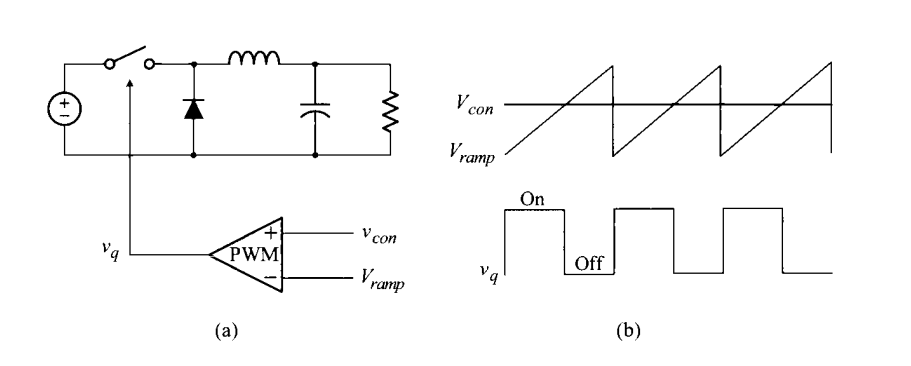
\includegraphics[width=0.8\linewidth]{2Grundlagen/141PWM.png}
    \caption{Schematische Darstellung eines PWM-Modulator. Quelle: \cite{choi2013pulsewidth}}
    \label{fig:PWM_converter}
\end{figure}


\section{Informationstechnologie}

\subsection{Einführung in Neuronale Netzwerke}
Neuronale Netzwerke bilden das rechnerische Grundgerüst für eine Vielzahl von Aufgaben in den Berei-chen maschinelles Lernen und künstliche Intelligenz. Sie sind von dem komplexen Netzwerk an Neuronen im menschlichen Gehirn inspiriert und versuchen, biologische Lernprozesse nachzuahmen \cite{aggarwal_neural_networks_2018}. In diesem Zusammenhang bieten sie ein robustes und flexibles Rahmenwerk zur Lösung komplexer Herausforderungen \cite{Goodfellow-et-al-2016}.

\subsubsection{Vorteile von Neuronalen Netzwerken}
Neuronale Netzwerke bieten mehrere entscheidende Vorteile, die ihren Einsatz in unterschiedlichen Anwendungsbereichen attraktiv machen:
\begin{itemize}
    \item \textbf{Parallelität:} Sie sind für die parallele Verarbeitung konzipiert und ermöglichen daher schnelle Berechnungen sowie Echtzeitverarbeitung.
    \item \textbf{Nichtlineare Funktionsapproximation:} Die Netzwerke sind besonders gut geeignet, nichtlineare Funktionen zu approximieren \cite{Goodfellow-et-al-2016}, was sie vielseitig einsetzbar macht.
    \item \textbf{Modellgeneralisierung:} Neuronale Netzwerke können aus einer begrenzten Datenmenge gene-ralisieren und somit präzise Vorhersagen für unbekannte Eingaben treffen.
\end{itemize}
Diese Vorteile bilden die Grundlage für ihre breite Anwendbarkeit, die im nächsten Abschnitt erläutert wird.

\subsubsection{Unterschied zwischen Biologischen und Künstlichen Neuronalen Netzwerken}
Künstliche neuronale Netzwerke bestehen aus rechnerischen Einheiten, den sogenannten Neuronen. Diese sind durch anpassbare Gewichtungen verbunden, die der Stärke synaptischer Verbindungen in biologischen Systemen ähneln. Lernen erfolgt durch die Anpassung dieser Gewichtungen, ähnlich wie sich die Stärken synaptischer Verbindungen in biologischen Systemen als Reaktion auf Reize ändern \cite{aggarwal_neural_networks_2018}.

\subsubsection{Deep Learning als Spezialisierung}
Deep Learning stellt einen spezialisierten Unterbereich des maschinellen Lernens dar, der neuronale Netzwerke mit drei oder mehr Schichten verwendet. Diese tiefen Netzwerke führen eine hierarchische Merkmalsextraktion durch, die es ihnen ermöglicht, immer komplexere Muster und Merkmale zu erkennen, während die Daten durch die Schichten fließen.

\subsubsection{Zusammenfassung und Ausblick}
Zusammenfassend bieten neuronale Netzwerke ein leistungsfähiges Rahmenwerk für eine Vielzahl von Aufgaben, von einfacher Mustererkennung bis hin zu komplexen Entscheidungsfindungsprozessen. Der Einsatz von mehrschichtigen Architekturen und nichtlinearen Aktivierungsfunktionen erweitert die Fähig-keiten traditioneller maschineller Lernalgorithmen \cite{aggarwal_neural_networks_2018}.

Mit dieser Grundlage werden die folgenden Abschnitte einen vertieften Einblick in die mathematischen Aspekte von neuronalen Netzwerken bieten. Insbesondere werden wir uns darauf konzentrieren, wie neuronale Netzwerke bei der Optimierung und Steuerung von PID-regulierten DC-Konvertern Anwendung finden. Dabei liegt der Fokus auf der Berücksichtigung von Alterungsprozessen und Abnutzung von Schaltungselementen wie Kapazitäten und Induktivitäten und wie diese Einflüsse mathematisch modelliert und optimiert werden können.

\subsection{Vorwärtspropagation in Neuronalen Netzwerken}
\label{sec: Forward Propagation}
Die Vorwärtspropagation ist ein wesentlicher Prozess in neuronalen Netzwerken, der die Übertragung von Eingabedaten durch die Netzwerkarchitektur ermöglicht, um die Ausgabe zu erzeugen \cite{russell2021ai}. 
Sie ist eine Abfolge von mathematischen Operationen, die Gewichtungen, Biases und Aktivierungsfunktionen beinhalten \cite{Chollet2021}.
Dieser Abschnitt zielt darauf ab, die Schlüsselelemente und mathematischen Grundlagen zu diskutieren, die die Vorwärtspropagation beeinflussen und stellt aktuelle Forschungsergebnisse und praktische Implikationen vor.
%
\subsubsection{Schicht-für-Schicht-Propagation}

Die Vorwärtspropagation beginnt bei den Eingabedaten \( X \), bezeichnet als \( A^{[0]} \). In jeder Schicht wird aus dem Ausgang \( A^{[l-1]} \) der vorherigen Schicht ein Vektor \( Z^{[l]} \) berechnet. Die Werte für jede nachfolgende Schicht \( A^{[l]} \) werden entsprechend der Gleichung (\ref{eq:forward}) ermittelt. Dieser Prozess wiederholt sich von Schicht zu Schicht und bildet das Kernstück der Vorwärtspropagation.
%
\begin{equation}
Z^{[l]} = W^{[l]} A^{[l-1]} + b^{[l]}
\label{eq:forward}
\end{equation}
%
%
%
%
\subsubsection{Aktivierungsfunktionen}
Aktivierungsfunktionen in neuronalen Netzen spielen eine entscheidende Rolle, indem sie die gewichtete Summe \( Z^{[l]} \) in einen aktivierten Ausgabewert \( A^{[l]} \) umwandeln. Diese Transformation wird typischerweise durch \( \sigma \) dargestellt, wie in der folgenden Gleichung gezeigt:
%
\begin{equation} \label{eq:activation_function}
A^{[l]} = \sigma(Z^{[l]})
\end{equation}
%
\begin{figure}[htbp]
  \centering
  \begin{subfigure}{0.45\textwidth}
    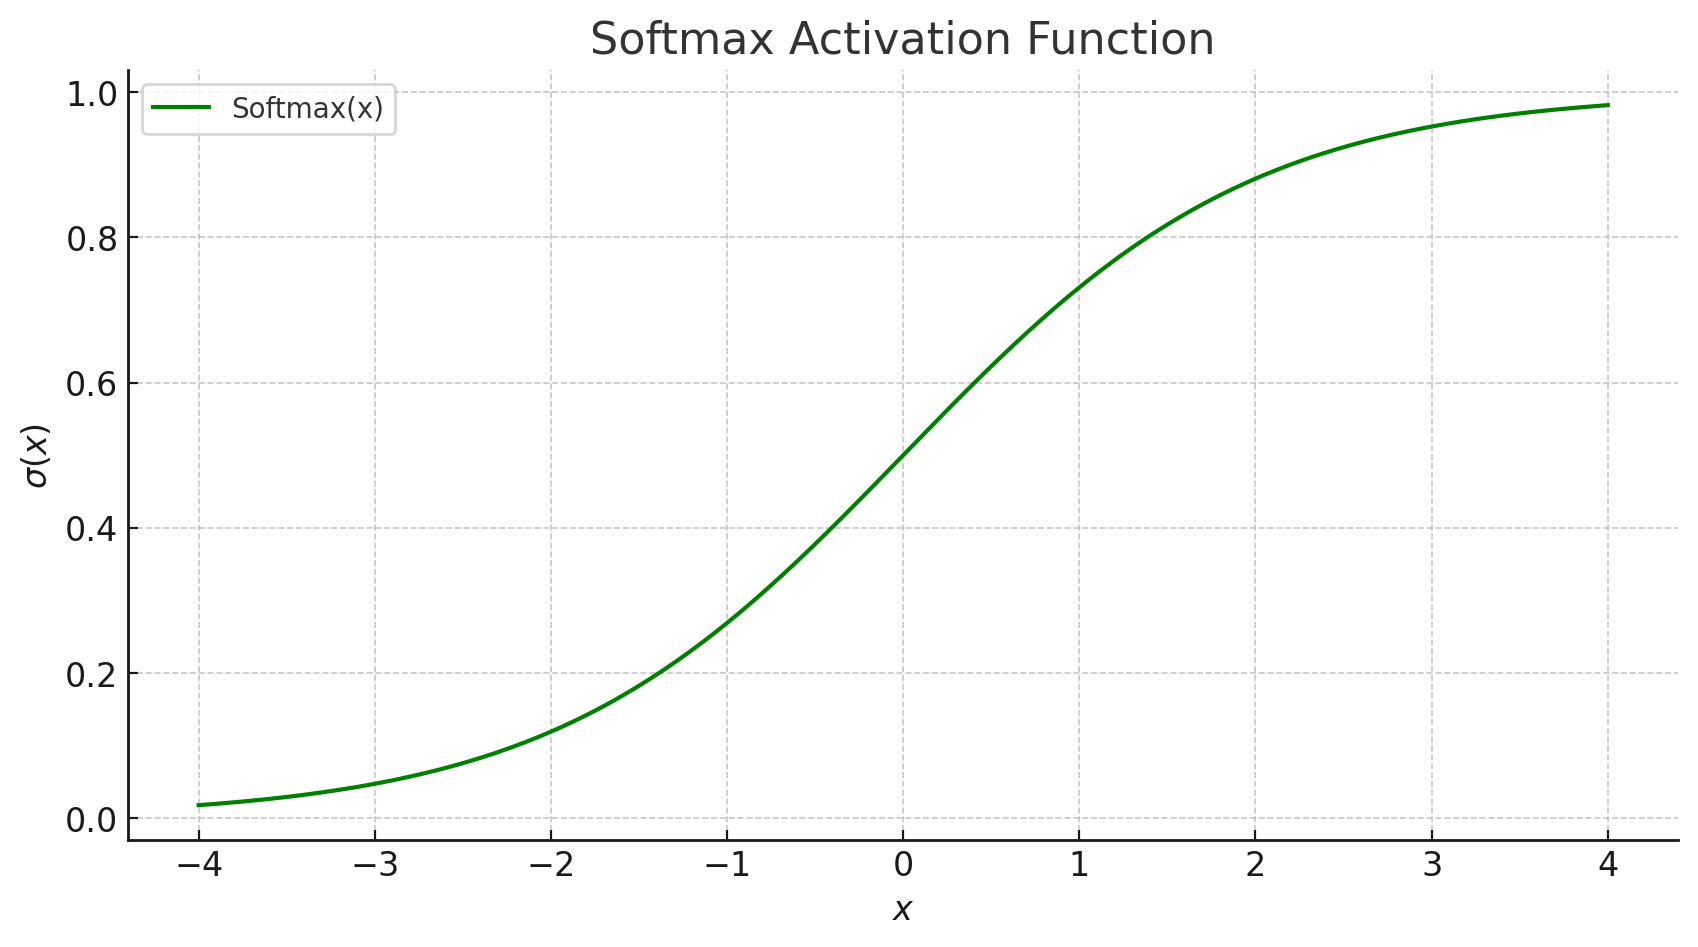
\includegraphics[width=\textwidth]{2Grundlagen/22SoftMax.png}
    \caption{Softmax-Funktion}
    \label{fig:softmax}
  \end{subfigure}
  \hfill
  \begin{subfigure}{0.45\textwidth}
    \includegraphics[width=\textwidth]{2Grundlagen/22ReLU.png}
    \caption{ReLU-Funktion}
    \label{fig:relu}
  \end{subfigure}
  \caption{Vergleich der Softmax- und ReLU-Aktivierungsfunktionen.}
\end{figure}
%
\paragraph{ReLU-Aktivierungsfunktion}
Die ReLU (Rectified Linear Unit) Aktivierungsfunktion, dargestellt in Abbildung \ref{fig:relu}, ist eine der am häufigsten verwendeten Aktivierungsfunktionen in neuronalen Netzen. Sie wird definiert als \( f(x) = \max(0, x) \) und ist besonders effektiv, um Nichtlinearitäten in den Daten zu modellieren.
%
\begin{equation} \label{eq:relu}
f(x) = \max(0, x)
\end{equation}
%

\paragraph{Softmax-Aktivierungsfunktion}
Die Softmax-Funktion ist eine Aktivierungsfunktion, die häufig in der Ausgabeschicht von Klassifizierungsnetzwerken verwendet wird. Sie wandelt einen Vektor von reellen Zahlen in Wahrscheinlichkeiten um. Die Formel für die Softmax-Funktion ist:
%
\begin{equation} \label{eq:softmax}
\text{Softmax}(z) = \frac{e^{z}}{\sum e^{z}}
\end{equation}
%
Hierbei steht \( e^{z} \) für den Exponentialwert jedes Elements im Vektor \( z \), und der Nenner ist die Summe aller Exponentialwerte im Vektor. Diese Umwandlung stellt sicher, dass die Ausgaben des Netzwerks als Wahrscheinlichkeiten interpretiert werden können, wobei die Summe aller Wahrscheinlichkeiten 1 ergibt.
%
%
\subsubsection{Gewichtsmatrix \( W^{[l]} \) und Bias-Vektor \( b^{[l]} \)}
Die Gewichtsmatrix für die Schicht \( l \) wird als \( W^{[l]} \) bezeichnet, und \( b^{[l]} \) ist der Bias-Vektor für dieselbe Schicht \cite{heaton_2012}. 
Diese Parameter werden während des Backpropagation-Prozesses trainiert, um den Fehler zwischen der vorhergesagten und der tatsächlichen Ausgabe zu minimieren \cite{aggarwal_neural_networks_2018}.
%
\begin{equation}
A^{[l]} = \sigma \left( 
\begin{pmatrix}
w_{1,1}^{[l-1,l]} & w_{1,2}^{[l-1,l]} & \cdots & w_{1,m}^{[l-1,l]} \\
w_{2,1}^{[l-1,l]} & w_{2,2}^{[l-1,l]} & \cdots & w_{2,m}^{[l-1,l]} \\
\vdots & \vdots & \ddots & \vdots \\
w_{n,1}^{[l-1,l]} & w_{n,2}^{[l-1,l]} & \cdots & w_{n,m}^{[l-1,l]}
\end{pmatrix}
\begin{pmatrix}
A_1^{[l-1]} \\
A_2^{[l-1]} \\
\vdots \\
A_m^{[l-1]}
\end{pmatrix}
+
\begin{pmatrix}
b_1^{[l]} \\
b_2^{[l]} \\
\vdots \\
b_n^{[l]}
\end{pmatrix}
\right)
	\label{eq:forward_big}
\end{equation}
%
\subsubsection{Matrix-Vektor-Operationen und Parallelität}
%
Die Gleichung (\ref{eq:forward_big}) illustriert die Verarbeitungsschritte während der Vorwärtspropagation in neuronalen Netzwerken. 
Eine besondere Stärke dieser Darstellung ist die Visualisierung der Matrix-Vektor-Operationen. 
Diese Operationen sind von Natur aus parallel, was bedeutet, dass sie mehrere Berechnungen gleichzeitig durchführen können. 
Dies zeigt sich besonders in der Matrixmultiplikation, bei der jede Zeile der Gewichtsmatrix gleichzeitig mit dem Aktivierungsvektor multipliziert wird.
%
In modernen Computerarchitekturen, insbesondere bei Grafikprozessoren (GPUs), kann diese inhärente Parallelität der Matrix-Operationen effektiv ausgenutzt werden, um die Berechnungsgeschwindigkeit erheblich zu steigern. 
Das bedeutet, dass die Berechnungen von \( Z^{[l]} \) und \( A^{[l]} \) simultan für alle Neuronen in Schicht \( l \) durchgeführt werden können. Dies ist ein entscheidender Vorteil, insbesondere in tiefen Netzwerken mit vielen Schichten und Neuronen.
%
Die Verwendung der Matrixnotation erleichtert nicht nur das Verständnis der Struktur und des Arbeitsablaufs eines neuronalen Netzwerks, sondern hebt auch die Möglichkeit hervor, leistungsstarke parallele Hardwarearchitekturen effizient zu nutzen.
%
%


\subsection{Einführung in die Backpropagation}

Backpropagation, oder auch "Rückpropagation des Fehlers", ist ein Optimierungsverfahren, das haupt-sächlich in der Ausbildung von künstlichen neuronalen Netzwerken verwendet wird. Das grundlegende Ziel der Backpropagation ist es, den Fehler, der während des Trainingsprozesses an der Ausgabeschicht berechnet wird, rückwärts durch das Netzwerk zu propagieren und durch Änderung der Gewichte zu minimieren. Dies ermöglicht die effiziente Anpassung der Gewichtungen und Bias-Werte des Netzwerks, um die Leistung zu verbessern.

\paragraph{Das Grundprinzip}

In einem neuronalen Netzwerk wird die Ausgabe durch eine Kette von Transformationen berechnet, die jeweils durch eine Schicht von Neuronen repräsentiert werden. Jedes Neuron in einer Schicht nimmt die Ausgaben der vorherigen Schicht auf, führt eine gewichtete Summe durch und wendet eine Aktivierungsfunktion an. Die endgültige Ausgabe wird dann mit dem tatsächlichen Zielwert verglichen, um einen Fehlerwert zu ermitteln. Dieser Fehler wird verwendet, um die Gewichtungen und Bias-Werte im Netzwerk so anzupassen, dass der Fehler minimiert wird.

\paragraph{Die Bedeutung der Kostenfunktion}
Die Kostenfunktion \( C_0 \), oft als Verlustfunktion bezeichnet, quantifiziert den Fehler zwischen den vorhergesagten Ausgaben und den tatsächlichen Zielwerten. Die Minimierung dieser Kostenfunktion ist das Hauptziel während des Trainingsprozesses, und Backpropagation ist das Schlüsselwerkzeug, das dabei hilft.

\paragraph{Rückpropagation in Neuronalen Netzwerken}
Zur Minimierung der Kostenfunktion \( C_0 \), die wie folgt definiert ist:

\begin{equation}
C_0 = \sum_{j=0}^{n_{L-1}} (a_j^{[L]} - y_j)^2
\label{eq:cost_function}
\end{equation}

wird die Technik der Rückpropagation verwendet. Das grundlegende Konzept besteht darin, den Fehler von der Ausgabeschicht rückwärts durch das Netzwerk zu propagieren. In Gleichung \ref{eq:cost_function} haben wir beispielhaft einen quadratischen Fehler als Kostenfunktion verwendet.

\cite{SuttonBarto2018}

\paragraph{Der Gradient des Fehlers in der Ausgabeschicht}

Die partielle Ableitung der Kostenfunktion \( C_0 \) in Bezug auf den Ausgabewert \( a_j^{[L]} \) wird durch folgende Formel definiert:

\begin{equation}
\label{eq:partial_derivative}
\frac{\partial C_0}{\partial a_j^{[L]}} = 2 \left( a_j^{[L]} - y_j \right)
\end{equation}

Dieser Ausdruck stellt den Gradienten des Fehlers in der Ausgabeschicht dar. Er gibt an, wie empfindlich die Kostenfunktion \( C_0 \) auf Änderungen in \( a_j^{[L]} \) reagiert. Dieser Wert wird zur Anpassung der Gewichtungen des Netzwerks während des Trainingsprozesses verwendet.

\paragraph{Fehler Rückpropagieren}

Die Ableitungen der Aktivierungsfunktion \( a_j^{[L]} \) und der linearen Kombination \( z_j^{[L]} \) sind:

\[
\frac{\partial a_j^{[L]}}{\partial z_j^{[L]}} = \sigma' \left( z_j^{[L]} \right)
\]
\[
\frac{\partial z_j^{[L]}}{\partial w_{jk}^{[L]}} = a_k^{[L-1]}
\]

\paragraph{Kettenregel Anwenden}

Nun kombinieren wir alle diese Teile mit der Kettenregel:

\[
\frac{\partial C_0}{\partial w_{jk}^{[L]}} = \frac{\partial C_0}{\partial a_j^{[L]}} \cdot \frac{\partial a_j^{[L]}}{\partial z_j^{[L]}} \cdot \frac{\partial z_j^{[L]}}{\partial w_{jk}^{[L]}}\]
\label{eq:Ketten Regel}

Durch Anwendung der Kettenregel erhalten wir:

\[
\frac{\partial C_0}{\partial w_{jk}^{[L]}} = 2 \left( a_j^{[L]} - y_j \right) \cdot \sigma' \left( z_j^{[L]} \right) \cdot a_k^{[L-1]}
\]

\paragraph{Gradienten der Kostenfunktion}

Der Gradient der Kostenfunktion \( C_0 \) in Bezug auf alle Gewichtungen wird durch folgende Matrix dargestellt:

\[
\nabla W^{[L]} C_0 = \left( 2 \left( a^{[L]} - y \right) \odot \sigma' \left( Z^{[L]} \right) \right) A^{[L-1]T}
\label{eq: gradient}
\]

Die Gradientenmatrix für die Gewichtungen in Bezug auf die Kostenfunktion \( C_0 \) kann in Matrixform dargestellt werden:

\[
\nabla_{W^{[L]}} C_0 = 
\begin{pmatrix}
2(a_1^{[L]} - y_1) \cdot \sigma' (z_1^{[L]}) \cdot a_1^{[L-1]} & \cdots & 2(a_1^{[L]} - y_1) \cdot \sigma' (z_1^{[L]}) \cdot a_m^{[L-1]} \\
2(a_2^{[L]} - y_2) \cdot \sigma' (z_2^{[L]}) \cdot a_1^{[L-1]} & \cdots & 2(a_2^{[L]} - y_2) \cdot \sigma' (z_2^{[L]}) \cdot a_m^{[L-1]} \\
\vdots & \ddots & \vdots \\
2(a_n^{[L]} - y_n) \cdot \sigma' (z_n^{[L]}) \cdot a_1^{[L-1]} & \cdots & 2(a_n^{[L]} - y_n) \cdot \sigma' (z_n^{[L]}) \cdot a_m^{[L-1]}

\label{eq: gradient matrix}
\end{pmatrix}
\]

Diese Matrix gibt die Änderungsrate der Kostenfunktion \( C_0 \) in Bezug auf das entsprechende Gewicht an.
\cite{SuttonBarto2018}

\paragraph{Schlussfolgerungen}
In diesem Kapitel wurde die Backpropagation-Technik ausführlich behandelt, ein Verfahren zur Optimierung von neuronalen Netzwerken. Mittels mathematischer Formeln wurde illustriert, wie der Fehler in der Ausgabeschicht des Netzwerks rückwärts propagiert wird, um eine Kostenfunktion \( C_0 \) zu minimieren. Besonders relevant ist die Anwendung der Kettenregel, die es erlaubt, die Änderungsrate der Kostenfunktion \( C_0 \) in Bezug auf die Gewichtungen zu berechnen. Diese Informationen sind entscheidend für die Anpassung der Gewichtungen und somit für die Verbesserung der Netzwerkleistung. Es sei darauf hingewiesen, dass nicht die einzigen Methoden sind, in der Praxis können je nach Anforderungen und Anwendungsfall auch andere Fehlerbestimmungsmethoden, Aktivierungsfunktionen und Netzwerkarchitekturen verwendet werden.


\subsection{Optimierungstechniken}

Die Wahl des Optimierers hat einen erheblichen Einfluss auf die Leistung eines neuronalen Netzwerks. Hier stellen wir einige gängige Optimierungsalgorithmen vor und erläutern den mathematischen Hintergrund des ADAM-Optimierers.

\paragraph{Stochastic Gradient Descent (SGD)}
\label{sec: Stochastisch Gredient Descent}

Der Stochastic Gradient Descent (SGD) ist ein fundamentales Optimierungsverfahren. 
Es unterscheidet sich von traditionellen Gradientenabstiegsverfahren dadurch, dass es nicht den gesamten Datensatz verwendet, um die Gradienten der Kostenfunktion zu jedem Schritt zu berechnen. 
Stattdessen nutzt der SGD nur eine zufällig ausgewählte Teilmenge oder sogar nur eine einzige Dateninstanz, um die Gradienten zu schätzen und die Modellgewichtungen anzupassen. 
Insbesondere im Rahmen des Reinforcement Learnings, wo zu jedem Zeitpunkt lediglich ein Teildatensatz verfügbar ist, erweist sich der SGD als besonders geeignet. 
Die stochastische Natur dieses Verfahrens kann helfen, aus lokalen Minima herauszukommen und zu einer besseren Konvergenz des Modells beizutragen.
\cite{klein_abbeel_cs188}

\paragraph{Momentum}

Momentum berücksichtigt sowohl den aktuellen Gradienten als auch die vorherigen Gradienten, um die Gewichtungen zu aktualisieren. Dadurch wird eine Art "Schwung" erzeugt, der dem Optimierer hilft, lokale Minima zu überwinden.

\paragraph{RMSprop}

Dieser Optimierer passt die Lernrate während des Trainings dynamisch an. Er verwendet den gleitenden Mittelwert der quadrierten Gradienten, um die Gewichtungen zu aktualisieren.

\paragraph{ADAM (Adaptive Moment Estimation)}
\label{sec: adam optimizer}

ADAM kombiniert die Vorteile von Momentum und RMSprop. Die Gewichtsaktualisierung in ADAM ist durch die folgende Gleichung definiert:

\begin{equation}
\theta_{t+1} = \theta_t - \alpha \times \frac{\hat{m}_t}{\sqrt{\hat{v}_t} + \epsilon}
\end{equation}

wobei \(\hat{m}_t\) und \(\hat{v}_t\) Schätzungen des ersten und zweiten Moments der Gradienten sind. Sie werden wie folgt berechnet:

\begin{equation}
\hat{m}_t = \frac{1}{1-\beta_1^t} \times m_t
\end{equation}
\begin{equation}
\hat{v}_t = \frac{1}{1-\beta_2^t} \times v_t
\end{equation}
\begin{equation}
m_t = \beta_1 \times m_{t-1} + (1-\beta_1) \times g_t
\end{equation}
\begin{equation}
v_t = \beta_2 \times v_{t-1} + (1-\beta_2) \times g_t^2
\end{equation}

wobei \(g_t\) der Gradient bei Schritt \(t\) ist, \(\beta_1\) und \(\beta_2\) Hyperparameter sind, und \(\alpha\) die Lernrate ist.
\cite{klein_abbeel_cs188}

\paragraph{Schlussfolgerungen}

Der Optimierer ist entscheidend für die Effizienz des Trainingsprozesses eines neuronalen Netzwerks. Der ADAM-Optimierer ist insbesondere eine ausgezeichnete Wahl für viele Anwendungen, da er sowohl die Vorteile von Momentum als auch von RMSprop kombiniert.


\subsection{Vermeidung von Overfitting in Neuronalen Netzen}
\label{sec: overfitting}

Overfitting ist ein kritisches Problem in der Anwendung neuronaler Netze, da es die Generalisierbarkeit des Modells auf neue Daten beeinträchtigt. 
Es tritt auf, wenn ein neuronales Netzwerk die Trainingsdaten "zu gut" lernt, einschließlich des Rauschens und der Ausreißer, und dadurch schlecht auf neue, unbekannte Daten generalisiert. 
Ein klares Anzeichen für Overfitting ist, wenn die Leistung auf dem Trainingsdatensatz steigt, während die Leistung auf dem Validierungsdatensatz stagniert oder abnimmt.
\cite{klein_abbeel_cs188}

\textbf{Strategien zur Vermeidung von Overfitting:}

\begin{enumerate}
    \item \textbf{Regularisierung}: Es gibt verschiedene Formen der Regularisierung wie L1 und L2, die durch die Einführung eines Regularisierungsterms in die Kostenfunktion die Modellkomplexität einschränken.
    \item \textbf{Dropout}: Einige Neuronen werden während des Trainings zufällig "ausgeschaltet", um das Modell daran zu hindern, sich zu stark auf bestimmte Merkmale zu verlassen.
    \item \textbf{Daten Augmentation}: Durch kleine Veränderungen der Eingabedaten kann der Trainingsdatensatz erweitert und die Generalisierungsfähigkeit des Modells verbessert werden.
    \item \textbf{Frühzeitiges Stoppen}: Das Training wird gestoppt, sobald die Leistung auf dem Validierungsdatensatz sich nicht mehr verbessert.
    \item \textbf{Stochastischer Gradientenabstieg}: Dieser Algorithmus kann als eine Form der Regularisierung betrachtet werden.
    \item \textbf{Vereinfachung der Architektur}: Reduzierung der Anzahl der Neuronen oder Schichten im Netzwerk.
    \item \textbf{Ensemble-Methoden}: Mehrere Modelle werden trainiert und ihre Vorhersagen kombiniert, um eine robustere Vorhersage zu erhalten. Dies kann als eine Form der Regularisierung betrachtet werden.
\end{enumerate}



\subsubsection{Regularisierung}

Die Kostenfunktion \( J(\theta) \) wird durch die Hinzufügung eines Regularisierungsterms erweitert:
\[
J(\theta) = \text{Ursprüngliche Kosten} + \frac{\lambda}{2m} \sum_{i=1}^{n} \theta_{i}^{2}
\]
Hierbei ist \( \lambda \) der Regularisierungsparameter und \( \theta \) sind die Gewichtungen des Modells.
\cite{klein_abbeel_cs188}


\subsubsection{Dropout}

Während des Trainings wird eine binäre Maske \( M \) mit einer Wahrscheinlichkeit \( p \) generiert und die Ausgabe eines jeden Layers wird mit dieser Maske multipliziert.

\subsubsection{Daten Augmentation}

Der Trainingsdatensatz \( D \) wird durch Transformationen \( T \) erweitert, um die Generalisierungsfähigkeit des Modells zu verbessern: 
\[
D' = D \cup T(D)
\]

\subsubsection{Frühzeitiges Stoppen}

Das Training wird gestoppt, sobald die Validierungsfehlerfunktion \( J_{\text{valid}}(\theta) \) anfängt zu steigen oder nicht mehr abnimmt.

\subsubsection{Vereinfachung der Architektur}

Die Anzahl der Schichten \( L \) oder Neuronen \( N \) wird reduziert, d.h., \( L' < L \) oder \( N' < N \).

\subsubsection{Ensemble-Methoden}

Mehrere Modelle \( f_{1}, f_{2}, \ldots, f_{n} \) werden trainiert und ihre Vorhersagen werden gemittelt oder anderweitig kombiniert:
\[
f_{\text{Ensemble}}(x) = \frac{1}{n} \sum_{i=1}^{n} f_{i}(x)
\]

\subsection{Vanishing-Gradient-Problem}

Neuronale Netze, insbesondere tiefe Architekturen, sind anfällig für das Problem der verschwindenden oder explodierenden Gradienten \cite{aggarwal_neural_networks_2018}. 
Während des Backpropagation-Prozesses können die Gradienten entweder zu klein werden, was als "Verschwinden" bezeichnet wird, oder zu groß, was als "Explodieren" bezeichnet wird. Beide Fälle erschweren das Training erheblich und können dazu führen, dass das Netzwerk nicht konvergiert oder instabil wird.

\subsubsection{Warum ist das ein Problem?}

Verschwindende Gradienten können dazu führen, dass die Gewichtsaktualisierungen für die ersten Schichten im Netzwerk minimal sind, wodurch das Netzwerk ineffizient trainiert wird. 
Explodierende Gradienten können dazu führen, dass die Gewichtsaktualisierungen zu groß werden, was das Training des Netzwerks destabilisiert \cite{aggarwal_neural_networks_2018}.

\subsubsection{Anpassung der Lernrate und optimierte Backpropagation-Techniken}

Eine Möglichkeit besteht darin, die Lernrate \( \alpha \) dynamisch während des Trainings anzupassen. Wenn der Gradient \( \nabla J \) einen bestimmten Schwellenwert überschreitet, könnte die Lernrate reduziert werden:

\[
\alpha = \alpha \times \text{decay}
\]

\subsubsection{Gradient Clipping}

Das sogenannte "Gradient Clipping" begrenzt den Gradienten \( \nabla J \) auf einen maximalen Wert \( C \) \cite{brunton2019data}:

\[
\nabla J = \min(\nabla J, C)
\]

\subsubsection{Architektur- und Ressourcenüberlegungen}

Die Wahl der Architektur und der Ressourcen spielt auch eine Rolle bei der Bewältigung von Gradientenproblemen. Ein gut durchdachtes Design kann helfen, das Problem der verschwindenden und explodierenden Gradienten zu mildern \cite{aggarwal_neural_networks_2018}.


\subsubsection{ReLU-Aktivierungsfunktion}

Die ReLU-Aktivierungsfunktion ist eine der am häufigsten verwendeten Aktivierungsfunktionen in neuronalen Netzen. Mathematisch wird die ReLU-Funktion wie folgt definiert:
\[
f(x) = \max(0, x)
\]


\paragraph{Warum ReLU beim Vanishing-Gradient-Problem hilft:}

Die ReLU-Aktivierungsfunktion hat mehrere Eigenschaften, die sie im Umgang mit dem Vanishing-Gradient-Problem nützlich machen:

\begin{itemize}
    \item \textbf{Lineare Aktivierung im positiven Bereich:} ReLU ist im positiven Bereich linear, wodurch der Gradient konstant gleich 1 bleibt. Dies erleichtert das Backpropagation-Verfahren, da der Gradient nicht beim Durchlaufen dieses Neurons verschwindet.
    
    \item \textbf{Sparsamkeit:} ReLU-Aktivierung führt dazu, dass einige Neuronen einen Ausgang von Null haben. Dies fördert die Sparsamkeit des Netzes, was dazu beitragen kann, Overfitting zu reduzieren.
    
    \item \textbf{Einfache Berechnung:} Im Vergleich zu anderen Aktivierungsfunktionen wie Sigmoid oder Tanh ist die ReLU-Funktion rechentechnisch weniger aufwendig, was zu schnelleren Trainingsschritten führt.
    
    \item \textbf{Nichtlinearität:} Obwohl sie in einem Bereich linear ist, ist die ReLU-Funktion insgesamt nichtlinear. Dies ermöglicht dem Netzwerk, komplexe Muster zu erfassen, während gleichzeitig das Vanishing-Gradient-Problem gemildert wird.
\end{itemize}


\subsubsection{Überwachung und manuelle Anpassung}

Es ist oft notwendig, das Verhalten des Netzwerks während des Trainings zu überwachen. Wenn Anzeichen für verschwindende oder explodierende Gradienten festgestellt werden, kann eine manuelle Anpassung der Architektur oder der Hyperparameter erforderlich sein.

\subsubsection{Anpassungen im aktuellen Ansatz}

In der vorliegenden Arbeit wurden bereits mehrere spezifische Methoden zur Bewältigung des Problems implementiert:


\begin{itemize}
    \item \textbf{Normalisierung des Rewards:} Der Reward-Wert \( R \) wurde angepasst:
    \[
    R_{\text{norm}} = \frac{R - \text{min}(R)}{\text{max}(R) - \text{min}(R)}
    \]
    
    \item \textbf{Normalisierung der Eingänge:} Die Eingangsdaten \( X \) wurden normalisiert:
    \[
    X_{\text{norm}} = \frac{X - \text{mean}(X)}{\text{std}(X)}
    \]
    
    \item \textbf{Verwendung von tanh:} Die Aktivierungsfunktion \(\tanh\) wurde verwendet, um die Ausgabe \( f(x) \) zu normalisieren:
    \[
    f(x) = \tanh(x)
    \]

    \item \textbf{ReLU-Aktivierungsfunktion}: Die Verwendung der ReLU-Aktivierungsfunktion (Rectified Linear Unit) kann dazu beitragen, das Vanishing-Gradient-Problem zu mildern und die Netzwerkeffizienz zu verbessern, was indirekt Overfitting verhindern kann.
\end{itemize}



\subsection{Bedeutung der Lernrate}
\label{sec: Learnign Rate}

Die Lernrate ist ein kritischer Hyperparameter, der die Geschwindigkeit der Modellanpassung steuert. Wie aus der Literatur bekannt ist, kann eine falsch gewählte Lernrate den Lernprozess verlangsamen oder sogar zu einer fehlgeschlagenen Konvergenz führen \cite{russell2021ai}. In ähnlicher Weise betont Heaton, dass die Wahl der Lernrate und des Momentums entscheidend für die Leistung des Trainings ist \cite{heaton_2012}.

\paragraph{subsectionHerausforderungen und Lösungsansätze}

Die Einstellung der Lernrate ist häufig ein Prozess des Ausprobierens, und die beste Methode zur Ermittlung der optimalen Lernrate ist nicht eindeutig. Goodfellow et al. erklären, dass die Lernrate das effektive Kapazitätsmodell in einer komplexeren Weise steuert als andere Hyperparameter \cite{Goodfellow-et-al-2016}. Daher ist es von entscheidender Bedeutung, sowohl das Training als auch den Testfehler zu überwachen, um zu diagnostizieren, ob das Modell unter- oder überangepasst ist.

\subsection{Bedeutung der Batch-Größe}
\label{sec: Batch}

Die Batch-Größe ist ein weiterer wichtiger Hyperparameter in der Ausbildung von neuronalen Netzwerken. Sie beeinflusst nicht nur die Rechenzeit, sondern auch die Modellgenauigkeit. Die Wahl der optimalen Batch-Größe ist ein Kompromiss zwischen Recheneffizienz und Modellqualität. Im Folgenden werden einige relevante Aspekte diskutiert.

\subsubsection{Berechnungseffizienz}
\begin{itemize}
    \item \textbf{Große Batches:} Eine große Batch-Größe ermöglicht es, viele Datenpunkte gleichzeitig durch das Netzwerk zu leiten, wodurch die Recheneffizienz erhöht wird. Minibatch-Stochastic Gradient Descent (SGD) ist in der Regel 10-mal schneller als Full-Batch-SGD, insbesondere bei Verwendung von parallelen Vektoroperationen auf modernen CPU- oder GPU-Architekturen \cite{russell2021ai}.
    
    \item \textbf{Kleine Batches:} Bei einer kleinen Batch-Größe wird weniger Speicher benötigt, und das Modell kann schneller auf den Daten trainieren, auch wenn dies zu einer höheren Varianz im Gradienten führen kann \cite{morales2020grokking}.
\end{itemize}

\subsubsection{Genauigkeit und Overfitting}
\begin{itemize}
    \item \textbf{Große Batches:} Größere Batches bieten in der Regel genauere Schätzungen des Gradienten, können jedoch zum Overfitting neigen, wenn nicht richtig reguliert \cite{Goodfellow-et-al-2016}.
    
    \item \textbf{Kleine Batches:} Die Verwendung kleinerer Batches kann eine regulierende Wirkung haben und kann das Generalisierungsvermögen des Modells verbessern \cite{Goodfellow-et-al-2016}.
\end{itemize}

\subsubsection{Hardware-Beschränkungen}
Die Größe der Batches kann auch durch die verfügbare Hardware begrenzt sein. Insbesondere ist der Arbeitsspeicher oft der begrenzende Faktor \cite{aggarwal_neural_networks_2018}.

\subsubsection{Empfehlungen}
Es ist eine gängige Praxis, Batch-Größen in Potenzen von 2 zu wählen, da dies häufig zu einer besseren Laufzeiteffizienz führt, besonders auf GPUs \cite{Goodfellow-et-al-2016}.

\section{Reinforcement Learning}
\subsection{Einleitung}

Nachdem wir die grundlegenden Konzepte neuronaler Netze und die Mechanismen von Forward- und Backpropagation ausführlich behandelt haben, wenden wir uns nun dem Thema Reinforcement Learning (RL) zu. Die zuvor erklärten neuronalen Netze dienen als Grundlage für RL und werden insbesondere als Funktionenapproximatoren verwendet, um Agenten zu simulieren und zu trainieren. In diesem Abschnitt beschäftigen wir uns mit den Kernkonzepten und Herausforderungen des Reinforcement Learning.

\paragraph{Grundlagen des Reinforcement Learning}

Reinforcement Learning ist ein maschinelles Lernverfahren, bei dem ein Agent in einer Umgebung agiert, um ein bestimmtes Ziel zu erreichen. Im Kern des Prozesses stehen zwei Hauptkomponenten: der Agent und die Umgebung (auch als Simulation bezeichnet). Der Agent nimmt den aktuellen Zustand der Umgebung wahr und trifft auf dieser Grundlage Entscheidungen, die als Aktionen bezeichnet werden \cite{morales2020grokking}. Diese Aktionen werden an die Umgebung übermittelt, welche daraufhin in einen neuen Zustand übergeht und dem Agenten eine Belohnung (engl. Reward) ausgibt.

Dieser Prozess kann in zwei Haupttypen von RL-Verfahren unterteilt werden: das modellbasierte und das modellfreie RL \cite{russell2021ai}. Bei modellbasierten Verfahren verwendet der Agent ein Übergangsmodell der Umgebung, um die Belohnungssignale zu interpretieren und Entscheidungen zu treffen. Im Gegensatz dazu lernt der Agent bei modellfreien Verfahren eine direktere Darstellung des Verhaltens, oft durch das Erlernen einer Q-Funktion, die die Qualität einer Aktion in einem bestimmten Zustand bewertet \cite{russell2021ai}.

Es ist wichtig zu betonen, dass RL-Agenten durch direkte Interaktion mit ihrer Umgebung lernen, ohne die Notwendigkeit einer beaufsichtigenden Instanz oder eines vollständigen Modells der Umgebung \cite{SuttonBarto2018}. Jede Interaktion, die als Zeitschritt bezeichnet wird, ermöglicht dem Agenten, seine Leistung durch Versuch und Irrtum zu verbessern \cite{morales2020grokking}.

Die Funktionsweise von RL kann als zyklisch beschrieben werden: Der Agent beobachtet die Umgebung, trifft eine Entscheidung, die Umgebung ändert ihren Zustand und gibt eine Belohnung zurück, und der neue Zustand wird dem Agenten wieder präsentiert. Durch diesen zyklischen Prozess lernt der Agent, optimale Entscheidungen zu treffen, um das gestellte Ziel zu erreichen.

\paragraph{Herausforderungen im RL}

RL stellt verschiedene Herausforderungen dar, die es von anderen maschinellen Lernmethoden unterscheiden. Ein wichtiger Aspekt ist die Sequenzialität der Entscheidungen. Die Agenten müssen nicht nur einmalige Entscheidungen treffen, sondern auch eine Sequenz von Aktionen planen, um ein optimales Ergebnis zu erzielen \cite{morales2020grokking}. Darüber hinaus müssen die Agenten in einer Umgebung mit Unsicherheit und Unvollkommenheit agieren, was den Einsatz von Methoden wie dem \textit{Markov-Entscheidungsprozess} erforderlich macht \cite{brunton2019data}.

\paragraph{Erweiterte Methoden und DDPG}

Der im nächsten Abschnitt behandelte DDPG (Deep Deterministic Policy Gradients) Algorithmus stellt eine fortschrittliche Methode in der Reinforcement-Learning-Domäne dar. Er übertrifft traditionellere Ansätze wie Policy Gradient oder Deep Q Networks (DQN) durch seine effizientere und schnellere Fähigkeit zur Identifizierung optimaler Policies \cite{morales2020grokking}.


\subsection{Markovsche Prozesse und deren Rolle im Reinforcement Learning}

Die Grundlage für viele Reinforcement Learning-Verfahren sind Markov-Entscheidungsprozesse (MDPs). Diese MDPs stellen eine stochastische Version des optimalen Steuerungsproblems dar, welches von Bellman eingeführt wurde \cite{SuttonBarto2018}. Grundlegend geht es bei einem MDP um Entscheidungen, die in einem Zustand getroffen werden, um eine maximale Belohnung in der Zukunft zu erzielen.

\paragraph{Grundlagen der Markovschen Prozesse}

Ein Markov-Entscheidungsprozess ist charakterisiert durch:
\begin{itemize}
\item Eine Menge von Zuständen, in denen sich das System befinden kann.
\item Eine Menge von Aktionen, die in jedem Zustand durchgeführt werden können.
\item Eine Belohnungsfunktion, die die sofortige Belohnung für den Übergang von einem Zustand in einen anderen definiert.
\item Eine Übergangsfunktion, die die Wahrscheinlichkeit beschreibt, von einem Zustand in einen anderen überzugehen, nachdem eine bestimmte Aktion ausgeführt wurde.
\end{itemize}

MDPs basieren auf der Markov-Eigenschaft, die besagt, dass die Zukunft nur vom gegenwärtigen Zustand abhängt und nicht von den vorhergehenden Zuständen. Das bedeutet, dass das System keine Erinnerung an frühere Zustände hat und die Zukunft unabhängig von der Vergangenheit ist, solange der aktuelle Zustand bekannt ist.

Ein entscheidendes Konzept in MDPs ist die sogenannte "Policy", eine Strategie, die festlegt, welche Aktion in jedem Zustand ausgeführt werden soll, um die kumulative Belohnung über die Zeit zu maximieren \cite{SuttonBarto2018}.

Ein einfacher Markov-Prozess kann als Zustandsdiagramm dargestellt werden. Im folgenden Beispiel gibt es drei Zustände: $S_1$, $S_2$, und $S_3$. 

\begin{figure}[h]
    \centering
    \begin{tikzpicture}[->,>=stealth',shorten >=1pt,auto,node distance=2.8cm,
                    semithick]
      % Zustände
      \node[state] (S1)              {$S_1$};
      \node[state] (S2) [right=of S1] {$S_2$};
      \node[state] (S3) [right=of S2] {$S_3$};

      % Übergänge mit Wahrscheinlichkeiten und Belohnungen
      \path (S1) edge [bend left] node[above] {0.7, +5} (S2)
            (S2) edge [bend left] node[above] {0.5, +3} (S3)
            (S3) edge [bend left] node[above] {0.8, +2} (S1)
            (S1) edge [loop left] node {0.3, +1} (S1)
            (S2) edge [loop above] node {0.5, +1} (S2)
            (S3) edge [loop right] node {0.2, +1} (S3);
    \end{tikzpicture}
    \caption{Beispiel für einen einfachen Markov-Prozess mit Übergangsbelohnungen}
    \label{fig:MarkovProzessBelohnungen}
\end{figure}

\paragraph{Legende}
\begin{itemize}
    \item Knoten: Zustände ($S_1$, $S_2$, $S_3$ usw.)
    \item Kanten: Erste Zahl ist die Übergangswahrscheinlichkeit, zweite Zahl ist die Belohnung für den Übergang
\end{itemize}

Im Diagramm repräsentieren die Knoten die Zustände und die Kanten repräsentieren die Übergangswahrscheinlichkeiten zwischen den Zuständen. 

\paragraph{Anwendung von Markovschen Prozessen im Reinforcement Learning}

Die Anwendung von MDPs im Reinforcement Learning ermöglicht es Agenten, optimale Strategien für komplexe Aufgaben zu erlernen. Dies geschieht durch die Interaktion des Agenten mit der Umgebung und die Anpassung seiner Strategie basierend auf den erhaltenen Belohnungen. Methoden wie "Policy Iteration" und "Value Iteration" werden verwendet, um optimale Policies zu ermitteln \cite{russell2021ai}.

Ein erweitertes Konzept von MDPs sind die POMDPs (Partially Observable Markov Decision Processes), bei denen der Agent nicht immer den genauen Zustand der Umgebung kennt. Dies führt zu komplexeren Strategien, bei denen der Agent versucht, Unsicherheiten durch Informationsbeschaffung zu reduzieren \cite{morales2020grokking}.

Abschließend können wir sagen, dass Markov-Entscheidungsprozesse ein zentrales Konzept im Reinforcement Learning darstellen, das es Agenten ermöglicht, in einer Vielzahl von Umgebungen effektive Strategien zu entwickeln.




\subsection{Das Multi-Armed Bandit Problem im Kontext der Degradation}

Das Multi-Armed Bandit Problem, häufig als ``Bandit Problem'' abgekürzt, stellt ein klassisches Dilemma in der Entscheidungsfindung unter Unsicherheit dar. Ursprünglich aus der Glücksspielwelt stammend, bei dem es darum geht, den gewinnbringendsten von mehreren Spielautomaten (den ``Banditen'') auszuwählen, hat dieses Problem vielfältige Anwendungen in den Bereichen künstliche Intelligenz und Maschinenlernen gefunden. Die Herausforderung liegt hierbei im Balancieren zwischen Exploration (Erkunden neuer oder weniger bekannter Aktionen) und Exploitation (Nutzen der besten bekannten Aktionen) \cite{SuttonBarto2018}.

In Bezug auf Degradationsvorgänge wird das Bandit Problem herangezogen, um den kontinuierlichen Verfall von Zuständen zu modellieren. Die Degradation, die sich über eine längere Zeitspanne erstreckt, lässt sich mittels eines markovschen Prozesses darstellen. Charakteristisch hierfür ist, dass trotz Durchführung einer Aktion der Zustandsübergang nur minimal ist, sodass es so wirkt, als würde das System in denselben Zustand zurückkehren.

Der gewählte Ansatz beinhaltet eine Sequenz von Zuständen \(S_1, \ldots, S_N\). In jedem dieser Zustände gibt es mehrere Aktionen, die den jeweiligen PID-Koeffizienten in diesem spezifischen Zustand repräsentieren. Interessanterweise wird durch die Modellierung der markovsche Prozess in ein Multi-Armed Bandit Problem überführt, sodass Zustände von \(S_0, \ldots, S_N\) existieren. Bei jeder Aktion innerhalb eines Zustands, charakterisiert durch drei PID-Parameter, gelangt das System wieder in denselben Zustand \cite{russell2021ai}.

\begin{figure}[h]
	\centering
	\begin{tikzpicture}[->,>=stealth',shorten >=1pt,auto,node distance=3.8cm,
		semithick]
		% Zustände
		\node[state] (Z1)              {\(Z_1\)};
		\node[state] (Z2) [right=of Z1] {\(Z_2\)};
		\node        (Zdots) [right=of Z2] {\(\cdots\)};
		\node[state] (Zn) [right=of Zdots] {\(Z_N\)};

		% Übergänge für Z1
		\path (Z1) edge [loop left] node[left] {$p_1$, $r_1$} 			(Z1)
		(Z1) edge [loop right] node[right] {\(\dots\)} 			(Z1)
		(Z1) edge [loop above] node[above] {$p_2$, $r_2$} 			(Z1)
		(Z1) edge [out=-45, in=-135, looseness=3] node[below] {$p_N$, $r_N$} 	(Z1);

		% Übergänge für Z2
		\path (Z2) edge [loop left] node[left] {$p_1$, $r_1$} 			(Z2)
		(Z2) edge [loop right] node[right] {\(\dots\)} 			(Z2)
		(Z2) edge [loop above] node[above] {$p_2$, $r_2$} 			(Z2)
		(Z2) edge [out=-45, in=-135, looseness=3] node[below] {$p_N$, $r_N$} 	(Z2);

		% Übergänge für ZN
		\path (Zn) edge [loop left] node[left] {$p_1$, $r_1$} 			(Zn)
		(Zn) edge [loop right] node[right] {\(\dots\)} 			(Zn)
		(Zn) edge [loop above] node[above] {$p_2$, $r_2$} 			(Zn)
		(Zn) edge [out=-45, in=-135, looseness=3] node[below] {$p_N$, $r_N$} 	(Zn);

	\end{tikzpicture}
	\caption{Erweiterte Darstellung des Multi-Armed Bandit Problems mit Zustandsaktionen von 1 bis N}
	\label{fig:ExtendedBanditDegradation}
\end{figure}

\paragraph{Legende}
\begin{itemize}
	\item Kanten: Erste Zahl \( p \) symbolisiert die Wahrscheinlichkeit der Aktion \( a \) 
	\item zweite Zahl \( r \) die Belohnung der Aktion.
\end{itemize}



\subsection{Markow-Entscheidungsprozesse und die Bellman-Gleichung}

Markow-Entscheidungsprozesse sind grundlegend für das Verständnis von Entscheidungsproblemen in stochastischen Umgebungen. Sie werden oft modelliert mit Zuständen \( s \), Aktionen \( a \), Zustandsübergängen \( P(s' | s, a) \) und Belohnungen \( R(s, a, s') \). Die Bellman-Gleichung dient als Eckpfeiler für die Lösung von MDPs und kann wie folgt geschrieben werden:
\[
U(s) = \max_{a \in A(s)} \sum_{s'} P(s' | s, a) \left[ R(s, a, s') + \gamma U(s') \right]
\label{eq: Bellman }
\]
Diese Gleichung erklärt uns im Wesentlichen den Nutzen eines Zustands \( s \) unter einer optimalen Policy. Sie repräsentiert die erwartete Summe der Belohnungen für einen Agenten, der von Zustand \( s \) startet und sich in der Zukunft optimal verhält \cite{russell2021ai}.

\subsubsection{Wenn \( \gamma = 0 \): Übergang zu Banditenproblemen}
\label{sec: discounted future reward}

Der Diskontfaktor \( \gamma \) ist wichtig, da er sofortige und zukünftige Belohnungen ausbalanciert. Wenn jedoch \( \gamma = 0 \), geraten wir in ein Szenario, das eher den Multi-Armed-Bandit-Problemen ähnelt, bei denen der Agent nur an sofortigen Belohnungen interessiert ist. In diesem Fall vereinfacht sich die Bellman-Gleichung zu:
\[
U(s) = \max_{a \in A(s)} \sum_{s'} P(s' | s, a) \left[ R(s, a, s') \right]
\]

Hier berücksichtigt der Agent nicht den zukünftigen Nutzen der Zustände \( s' \), in die er übergehen könnte. Er maximiert nur seine sofortige Belohnung, was das Problem zu einem Einzelschritt-Entscheidungsproblem macht \cite{SuttonBarto2018}.

\subsection{Policy-Based Reinforcement Learning}

Policy-Based Reinforcement Learning konzentriert sich auf das direkte Lernen einer Policy \(\pi(s)\), die Zuständen \(s\) Aktionen \(a\) zuordnet. Diese Methoden, insbesondere Policy Gradient Ansätze, sind effektiv in Umgebungen mit diskreten und kontinuierlichen Aktionsräumen.\cite{SuttonBarto2018}.

\paragraph{Mathematische Grundlagen}
Die Aktualisierung der Policy-Parameter \(\theta\) erfolgt anhand des Policy Gradient Ansatzes, wie in der folgenden Gleichung dargestellt:
\begin{equation} 
\nabla_{\theta} J(\theta) = \mathbb{E}_{\pi} \left[ \nabla_{\theta} \log \pi(a | s; \theta) \cdot R(s, a) \right]
		\label{eq:policy_gradient}
\end{equation}

Hierbei ist \(J(\theta)\) die zu maximierende Zielfunktion, \(R(s, a)\) die Belohnung und \(\theta\) die Policy-Parameter \cite{russell2021ai}. Die Aktionen werden basierend auf der Wahrscheinlichkeitsverteilung der Policy, häufig modelliert durch eine Softmax-Funktion, ausgewählt \cite{russell2021ai}, wie in Gleichung \ref{eq:relu} dargestellt.

\paragraph{Visuelle Darstellung der Policy-Werte}
Ein Beispiel für eine trainierte Policy in einem einfachen Rasterumfeld zeigt Abbildung \ref{fig:trained_policy}. Jede Zelle des Rasters repräsentiert einen Zustand mit einem zugeordneten Wert, der die erwartete zukünftige Belohnung unter dieser Policy anzeigt. Pfeile in den Zellen deuten die von der Policy gewählten Aktionen an, wobei die grünen Zellen eine positive Belohnung (Zielzustände) und die rote Zelle eine negative Belohnung (Strafzustände) symbolisieren.

\begin{figure}[h]
\centering
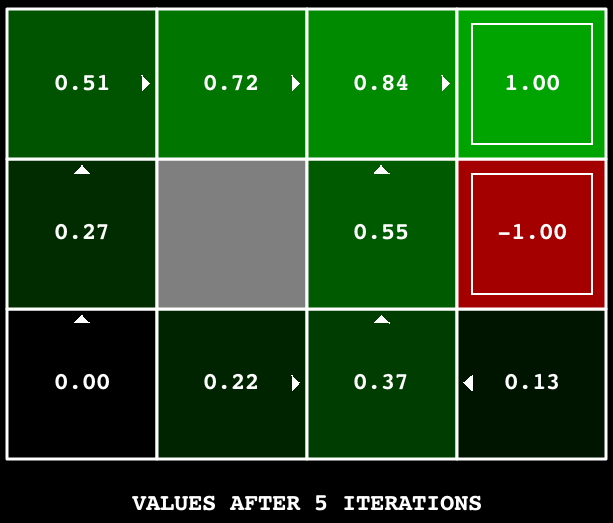
\includegraphics[width=0.5\textwidth]{2Grundlagen/33Policy.png}
\caption{Trainierte Policy nach 5 Iterationen. Jede Zelle zeigt den geschätzten Wert des Zustands und die von der Policy empfohlene Aktion. Grüne Zellen kennzeichnen positive Belohnungen, die rote Zelle kennzeichnet eine negative Belohnung.}
\label{fig:trained_policy}
  \cite{klein_abbeel_cs188}
\end{figure}
%
\paragraph{Pseudocode}
Die Aktualisierung der Policy-Parameter, wie in Gleichung \ref{eq:policy_gradient} beschrieben, erfolgt nach dem folgenden Schema:
\begin{algorithmic}
\STATE Initialisiere die Policy-Parameter \(\theta\)
\STATE Setze die Lernrate \(\alpha\)
\FOR{jede Episode}
    \STATE Initialisiere den Zustand \(s\)
    \WHILE{\(s\) kein terminaler Zustand ist}
        \STATE Wähle Aktion \(a\) basierend auf der aktuellen Policy \(\pi(s; \theta)\)
        \STATE Führe Aktion \(a\) aus, beobachte Belohnung \(r\) und neuen Zustand \(s'\)
        \STATE Aktualisiere die Policy-Parameter:
        \STATE \(\theta \leftarrow \theta + \alpha \nabla_{\theta} \log \pi(a | s; \theta) \cdot r\)
        \STATE \(s \leftarrow s'\)  \# Wechsel zum neuen Zustand
    \ENDWHILE
\ENDFOR
\end{algorithmic}

\paragraph{Wahl der Aktion in Policy-Based-Methoden}

In Policy-Based Reinforcement Learning-Methoden erfolgt die Aktionsermittlung basierend auf einer Wahrscheinlichkeitsverteilung der aktuellen Policy \(\pi(s; \theta)\), oft repräsentiert durch die Softmax-Funktion ,\ref{fig:softmax} wie in Abbildung \ref{eq:softmax} illustriert \cite{russell2021ai}. Besonders effektiv sind diese Methoden in komplexen Umgebungen, wo lineare oder einfache Beziehungen zwischen Zuständen, Aktionen und Belohnungen fehlen \cite{SuttonBarto2018}. Die direkte Optimierung der Policy ohne separate Value-Funktion bietet Vorteile, stellt jedoch eine Herausforderung dar, da eine umfangreiche Erkundung des Zustandsraums für die Konvergenz notwendig ist \cite{morales2020grokking}. Ein häufiger Ansatz zur Aktionsermittlung in diskreten Räumen ist der Epsilon-Greedy-Algorithmus \ref{eq:epsilon_greedy}, der die Balance zwischen Exploration und Exploitation hält \cite{SuttonBarto2018}.

\paragraph{Einschränkungen von Policy-Based-Methoden}
%
Policy-Based Methoden im Reinforcement Learning, effektiv in diskreten und kontinuierlichen Aktionsräumen, stoßen in komplexen Umgebungen an Grenzen. Ihre Hauptherausforderung ist die benötigte umfangreiche Erkundung des Zustandsraums für die Konvergenz, was in kostspieligen oder riskanten Szenarien praktisch problematisch sein kann \cite{SuttonBarto2018}. Zudem konvergieren sie langsamer als Value-Based-Methoden, besonders in Umgebungen mit vielen Zuständen oder hoher Dimensionalität, da die direkte Optimierung der Policy ohne konkrete Werteschätzungen aufwendiger ist \cite{SuttonBarto2018}. Diese Methoden sind zwar theoretisch für kontinuierliche Aktionsräume geeignet, ihre Effektivität kann jedoch in der Praxis durch feingranulare Aktionen und schwer abschätzbare Konsequenzen begrenzt sein.

\subsection{Q-Learning}
%
Q-Learning ist ein modellfreier Algorithmus für das Erlernen der optimalen Entscheidungsfindung in der RL-Umgebungen. Der Algorithmus wurde 1989 von Chris Watkins in seiner Doktorarbeit eingeführt und hat sich als einer der beliebtesten Algorithmen im Bereich des RL-Umgebungen etabliert \cite{morales2020grokking}. Anstelle eines Übergangsmodells wird eine .direkt aktualisiert, die die Qualität jeder möglichen Aktion in einem bestimmten Zustand repräsentiert \cite{russell2021ai}.
%
\paragraph{Mathematische Grundlagen}
%
Die Aktualisierung der Q-Werte \( Q(s, a) \) erfolgt anhand der Bellman-Gleichung:
\[
		Q(s, a) \leftarrow Q(s, a) + \alpha \left[ R(s, a, s') + \gamma \max_{a'} Q(s', a') - Q(s, a) \right]
		\label{eq: update q learning}
\]
wobei \( s \) der aktuelle Zustand, \( a \) die gewählte Aktion, \( s' \) der neue Zustand, \( R(s, a, s') \) die unmittelbare Belohnung, \( \alpha \) die Lernrate und \( \gamma \) der Abschlagfaktor ist \cite{russell2021ai}.
%
\paragraph{Pseudocode}
Der Pseudocode für den Q-Learning-Algorithmus könnte wie folgt aussehen:\\
%
\begin{algorithmic}
		\STATE Initialize $Q(s, a)$ for all states and actions
		\STATE Set parameters $\alpha$ and $\gamma$
		%
		\FOR{each episode}
		\STATE Initialize state $s$
		\WHILE{$s$ is not a terminal state}
		\STATE Choose action $a$ based on policy (e.g., epsilon-greedy) derived from $Q(s, a)$
		\STATE Take action $a$, observe reward $r$ and new state $s'$
		\STATE Update Q-value:
		\STATE $Q(s, a) \gets Q(s, a) + \alpha \cdot (r + \gamma \cdot \max(Q(s', a')) - Q(s, a))$
		\STATE $s \gets s'$  \# Move to the new state
		\ENDWHILE
		\ENDFOR
\end{algorithmic}
%
Dieser Algorithmus benötigt keine Modellierung der Umgebung und ist daher besonders nützlich in komplexen oder unbekannten Umgebungen \cite{morales2020grokking}. Es handelt sich um ein "Off-Policy"-Verfahren, was bedeutet, dass es die optimale Q-Funktion lernt, unabhängig von der während des Lernens verwendeten Richtlinie \cite{morales2020grokking}.

Die sogenannte Heatmap in Abbildung \ref{fig:grid_world_q_learning} visualisiert die Q-Werte, die der Agent in jedem Zustand der Rasterwelt zugewiesen hat. Die Farbgebung illustriert, wie Q-Learning durch Interaktion mit der Umgebung diese Werte optimiert, indem es Belohnungen maximiert, was durch die Bellman-Gleichung mathematisch fundiert ist. Dieser Prozess des stetigen Aktualisierens der Q-Werte, die die erwarteten zukünftigen Belohnungen für jede Aktion in jedem Zustand repräsentieren, zeigt die modellfreie Natur des Q-Learning-Algorithmus und seine Fähigkeit, optimale Strategien zu erlernen, auch wenn die genaue Dynamik der Umgebung unbekannt ist. Die in Abbildung \ref{fig:grid_world_q_learning} dargestellten Informationen ergänzen somit die theoretischen Konzepte, die in diesem Abschnitt diskutiert wurden, indem sie ein konkretes Beispiel für die Anwendung von Q-Learning in einer simulierten Umgebung bieten \cite{klein_abbeel_cs188}.
%
%
\begin{figure}[htbp]
		\centering
		% erstes Bild
		\begin{minipage}[b]{0.48\linewidth}
				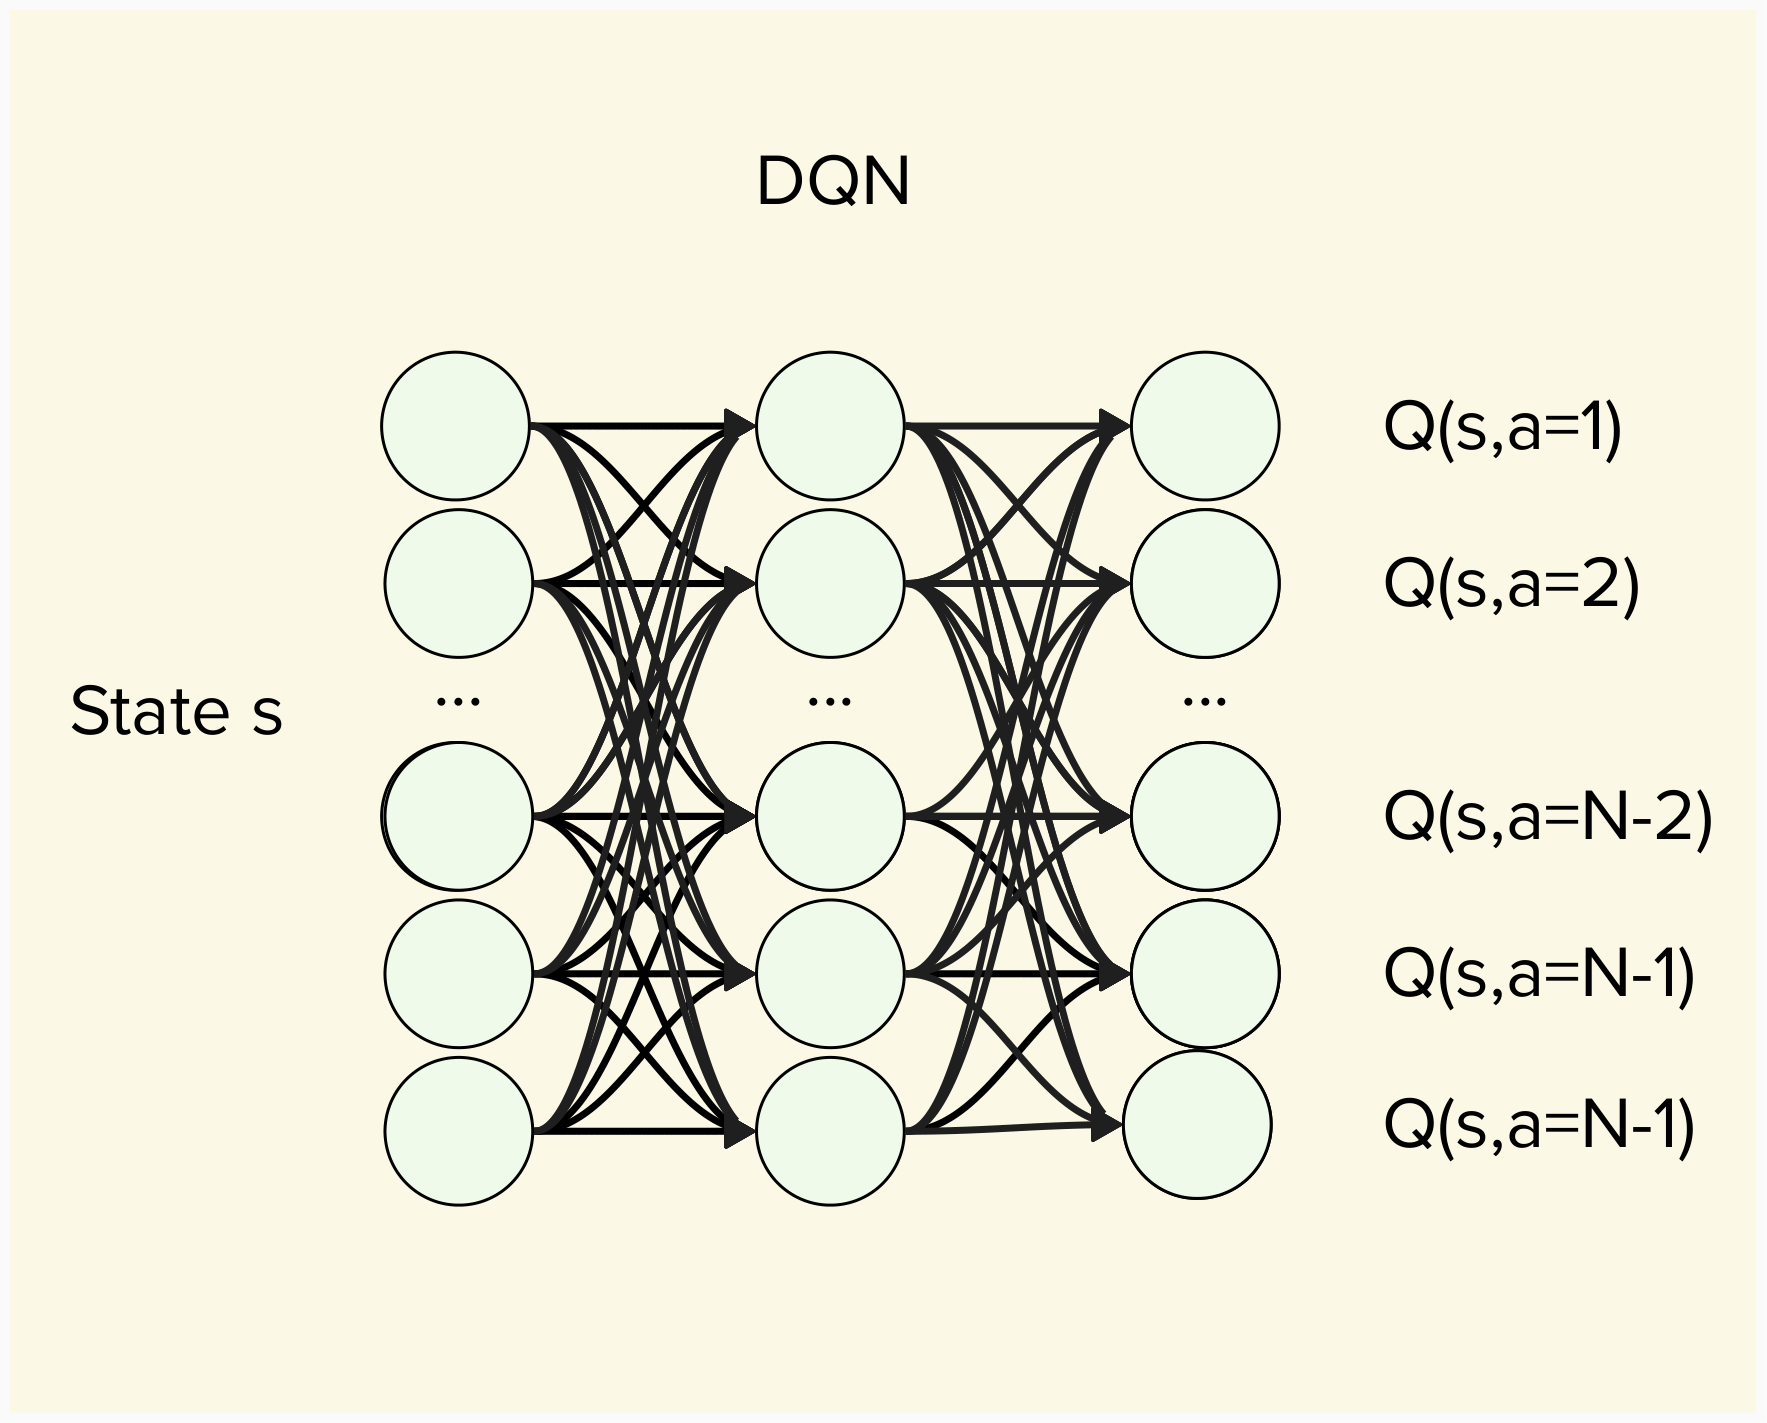
\includegraphics[width=\linewidth]{2Grundlagen/33grid_world_q_learning.png}
				\caption{Schematische Darstellung eines Deep Q-Networks (DQN), das für RL-Umgebungen verwendet wird.}
				\label{fig:dqn}
		\end{minipage}
		\hfill % Dies sorgt für Abstand zwischen den Bildern
		% zweites Bild, angehoben um 50pt
		\raisebox{1pt}[0pt][0pt]{%
				\begin{minipage}[b]{0.48\linewidth}
						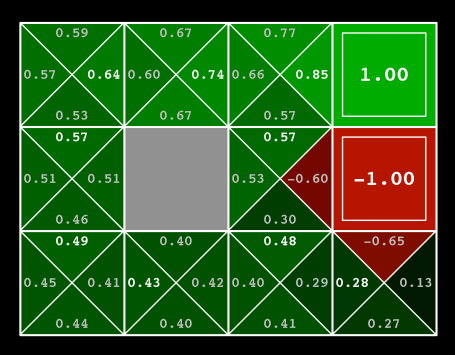
\includegraphics[width=\linewidth]{2Grundlagen/33Q_Values.png}
						\caption{Darstellung einer Heatmap von Q-Werten in einer Rasterwelt.}
						\label{fig:grid_world_q_learning}
						\cite{klein_abbeel_cs188}
				\end{minipage}%
				}
\end{figure}

\paragraph{Das $\epsilon$-greedy Verfahren im RL-Umgebungen}
\begin{equation}
		a = 
		\begin{cases}
				\underset{a}{\mathrm{argmax}}\ Q(s,a) & \text{mit Wahrscheinlichkeit } 1 - \epsilon, \\
				\text{eine zufällige Aktion} & \text{mit Wahrscheinlichkeit } \epsilon.
		\end{cases}
		\label{eq:epsilon_greedy}
\end{equation}


\paragraph{Deep Q-Learning}

Der Kernunterschied zwischen Q-Learning und Deep Q-Learning (DQL) liegt in der Methodik der Approximation der Q-Werte, die im Zentrum beider Ansätze steht. Klassisches Q-Learning nutzt eine Q-Tabelle, um Werte für Zustands-Aktions-Paare zu speichern, was bei einer begrenzten Anzahl von Zuständen und Aktionen gut funktioniert. Jedoch wird diese Methode unpraktikabel in komplexen, hochdimensionalen Umgebungen. Hier kommt DQL ins Spiel, das neuronale Netze verwendet, um diese Werte effizient zu schätzen \cite{morales2020grokking}. 

Wie Abbildung \ref{fig:dqn} veranschaulicht, ermöglicht die Verwendung von tiefen neuronalen Netzen in einem Deep Q-Network (DQN), eine effektive Handhabung von Situationen mit einer hohen Anzahl von Zuständen, die über das Fassungsvermögen einer herkömmlichen Q-Tabelle hinausgehen. Diese fortgeschrittenen Netzwerke sind in der Lage, direkt aus rohen visuellen Eingaben zu lernen und entwickeln im Laufe der Zeit eine verfeinerte Q-Funktion, welche die Entscheidungsfindung des Agenten verbessert. Diese Verbesserung wird durch den Einsatz von Deep Learning-Techniken erreicht, die es dem DQN ermöglichen, abstrakte Repräsentationen für die Entscheidungsfindung zu lernen und zu nutzen, was eine signifikante Verbesserung gegenüber traditionellen Q-Learning-Techniken darstellt \cite{brunton2019data}.


\paragraph{Exploration versus Exploitation}
\label{sec: Exploration versus Exploitation}

Die Balance zwischen Exploration und Exploitation ist essentiell für die Effektivität von lernenden Agenten im Q-Learning, die sich im Laufe ihrer Interaktion mit der Umgebung stetig anpassen müssen.

Durch die Anwendung des \(\epsilon\)-greedy Verfahrens \ref{eq:epsilon_greedy} im RL-Umgebungen wird ein Kompromiss zwischen der Erforschung unbekannter Aktionen und der Ausnutzung bekannter Strategien gefunden. Dies ermöglicht es einem Agenten, sowohl Neues zu entdecken als auch bewährte Taktiken einzusetzen, um den unmittelbaren Gewinn zu maximieren \cite{SuttonBarto2018}.

Die Dynamik von \(\epsilon\) spielt eine wichtige Rolle: Zu Beginn des Lernprozesses fördert ein höheres \(\epsilon\) die Exploration. Mit zunehmender Erfahrung sollte \(\epsilon\) jedoch sinken, was den Übergang zur gezielten Exploitation bewirkt \cite{morales2020grokking}.

Simulated Annealing erlaubt es, unter bestimmten Bedingungen auch Verschlechterungen des aktuellen Zustands zu akzeptieren. Dies wird durch die "Temperatur", einen Metaparameter, ermöglicht, der analog zur physikalischen Temperatur in der Metallurgie die Wahrscheinlichkeit für das Akzeptieren schlechterer Zustände bestimmt \cite{russell2021ai}. Im Metallurgieprozess bezeichnet Annealing den Vorgang, bei dem Metalle und Glas erhitzt und dann langsam abgekühlt werden, um eine stabile, kristalline Struktur zu erlangen \cite{russell2021ai}.
\label{sec:Simulated Annealing}

Simulated Annealing beginnt mit einer hohen "Temperatur", die es dem Algorithmus ermöglicht, lokale Minima zu verlassen, indem temporär schlechtere Lösungen akzeptiert werden. Mit der Zeit wird die Temperatur reduziert, wodurch der Algorithmus sich einem globalen Optimum annähert. Eine ähnliche Vorgehensweise findet sich im \(\epsilon\)-greedy Verfahren, bei dem \(\epsilon\), ein Parameter, der die Exploration im Verhältnis zur Exploitation steuert, allmählich verringert wird. Wie bei der kontrollierten Abkühlung, die Materialien in eine stabilere Struktur überführt, reduziert das Senken von \(\epsilon\) im Laufe der Zeit die Neigung zur Erkundung und fördert eine zunehmend spezialisierte Nutzung der besten bekannten Handlungsoptionen \cite{russell2021ai}.

Durch die methodische Reduktion von \(\epsilon\) wird vermieden, dass der Lernprozess in suboptimalen Lösungen verharrt. Stattdessen bleibt die Möglichkeit erhalten, bessere Aktionen zu entdecken und zu nutzen, was zu einer effektiveren und effizienteren Suche führt \cite{russell2021ai}.

Die Feinabstimmung von \(\epsilon\) ist entscheidend, da eine nicht angepasste Rate entweder zu wenig Exploration oder zu verzögerter Optimierung führen kann \cite{morales2020grokking}.



\paragraph{Replay Buffers}
\label{sec:Replay Buffers}

Replay Buffers verringern die Korrelation aufeinanderfolgender Erfahrungen und fördern so die Stabilität beim Lernen von RL-Agenten \cite{morales2020grokking}. Sie speichern eine Sammlung von Erfahrungstupeln aus unterschiedlichen Policies und Trajektorien und ermöglichen eine effektivere Trainingsmethode durch zufällige Stichprobenziehung, was die Netzwerkaktualisierungen diversifiziert \cite{morales2020grokking}.

Mathematisch wird der Replay Buffer wie folgt definiert \cite{morales2020grokking}:
\begin{equation}
		\mathcal{D} = \{ e_t = (s_t, a_t, r_t, s_{t+1}, d_t) \mid t \in \{1, \ldots, T\} \}
\end{equation}

Sampling aus dem Replay Buffer erfolgt per Zufallsauswahl ohne Zurücklegen, um einen Minibatch von \( n \) Erfahrungen zu generieren:
\begin{equation}
		\mathcal{B} = \{ e_i \mid e_i \in \mathcal{D}, i \in \mathcal{I} \}
		\label{eq:replay buffer}
\end{equation}
wobei \( \mathcal{I} \subset \{1, \ldots, T\}, \quad |\mathcal{I}| = n \).

Die Kapazität des Buffers und das gleichförmige Sampling sorgen für ein diversifiziertes Lernen und vermeiden lokale Optima \cite{morales2020grokking}. Die effektive Nutzung eines Replay Buffers erfordert eine ausreichende Kapazität, die typischerweise zwischen 10.000 und 1.000.000 Erfahrungen variiert \cite{morales2020grokking}. Ein priorisiertes Sampling könnte eine intelligentere Auswahlmethode darstellen, die eine ausgewogenere Lernumgebung fördert \cite{morales2020grokking}.
%
\paragraph{Fortgeschrittene Anpassungsfähigkeit und Lernmechanismen in Tiefen Q-Netzwerken (DQN) und ihre Bedeutung in der Entwicklung Künstlicher Intelligenz}
%
Die Tiefen Q-Netzwerke (DQN) haben sich als revolutionär in der Landschaft des maschinellen Lernens erwiesen. Mit ihrer Fähigkeit, eine Policy direkt aus rohen Pixeln zu lernen, signalisierte das DQN einen Wendepunkt in der Forschung von Reinforcement Learning (RL). Wie in \cite{morales2020grokking} dargestellt, hat das DQN die Tür zu einer Vielzahl von Forschungsinnovationen geöffnet und zu Beginn eine Leistung demonstriert, die auf menschenähnlichem Niveau auf einem Atari-Benchmark lag. Es ist erwähnenswert, dass trotz der Weiterentwicklungen DQN in seiner ursprünglichen Form nicht mehr als Primärwahl für aktuelle Anwendungen gilt, es bleibt jedoch ein Schlüsselelement unter den bestperformenden DRL-Agenten.
%
Die Fähigkeit des DQN, optimale Policy aus einer komplexen Umgebung wie der eines Atari-Spiels zu extrahieren, ist vergleichbar mit der Navigation in einem sich ständig verändernden Labyrinth, auf der Suche nach dem optimalen Weg (\cite{russell2021ai}). Die Anwendung der neuronalen Netze, speziell die tiefen Architekturen, ermöglicht es dem DQN, abstrakte Repräsentationen zu erlernen und diese für die Entscheidungsfindung zu nutzen.
%
Eine Herausforderung, auf die in \cite{SuttonBarto2018} hingewiesen wird, ist jedoch, dass DQN bei Spielen wie Montezuma's Revenge, die tiefergehende Planung erfordern, an seine Grenzen stößt. Obwohl DQN wesentliche Fortschritte im maschinellen Lernen gezeigt hat, verbleiben Herausforderungen in seiner Fähigkeit, komplexe Planungsaufgaben zu meistern.
%
Das beeindruckende Potenzial der DQN-Methode wurde weiterhin durch das System AlphaGo von DeepMind illustriert, das tiefes RL verwendete, um menschliche Experten im Go-Spiel zu schlagen, einem Spiel, das für seine immense Anzahl möglicher Positionen bekannt ist und weit über das hinausgeht, was traditionelle Spiele bieten (\cite{russell2021ai}). Dies bestätigt, dass trotz der Herausforderungen, DQN und seine Weiterentwicklungen ein hohes Maß an Anpassungsfähigkeit und Lernfähigkeit aufweisen, das es ihnen ermöglicht, auch in komplexen Umgebungen zu bestehen.
%
Im Licht dieser Quellen lässt sich zusammenfassen, dass DQN und dessen Erweiterungen ein bedeutsames Fundament für die Entwicklung von lernenden Agenten bieten, das sowohl die Forschung als auch praktische Anwendungen weiterhin beeinflusst.
%

\paragraph{Grenzen von Deep Q-Learning in kontinuierlichen Aktionsräumen}
Deep Q-Learning zeigt zwar in diskreten Aktionsräumen eine beeindruckende Leistung, stößt aber bei der Diskretisierung von kontinuierlichen Aktionsräumen auf bedeutende Herausforderungen. Die Notwendigkeit, kontinuierliche Aktionen in diskrete Schritte zu unterteilen, kann zu einem Verlust an Präzision und einer Verschlechterung der Leistung führen, insbesondere in Bereichen wie der Robotik, wo fein abgestimmte Kontrollaktionen erforderlich sind. Diese Limitation kann auch durch die Verwendung von Bewegungsprimitiven anstatt von niederstufigen Aktionen gemildert werden, was zwar das Lernen beschleunigt, aber die Bandbreite der Verhaltensweisen, die der Roboter lernen kann, einschränkt \cite{russell2021ai}. Weiterhin kann die Diskretisierung zu instabilen Steuerungsvorgängen führen, was insbesondere in sicherheitskritischen Systemen wie autonomen Fahrzeugen problematisch ist \cite{Wu2018AggregatedMultiDDPG}. Zusätzlich wird die Anwendung von Deep Q-Learning durch die erhöhte Berechnungskomplexität und Schwierigkeiten bei der Konvergenz in großen Zustandsräumen eingeschränkt \cite{russell2021ai}.




\subsection{Deep Deterministick Policy Gradienten (DDPG)}

Während das Deep Q-Network (DQN) für jeden Zustand s eine Bewertung aller möglichen Aktionen a liefert, wie in Abbildung \ref{fig:dqn} illustriert, stößt es in kontinuierlichen Aktionsräumen an seine Grenzen. Die Unzulänglichkeit von DQN in solchen Szenarien -- da die Bewertung einer unendlichen Anzahl von Aktionen nicht praktikabel ist -- führt uns zu fortgeschritteneren Methoden wie dem Deep Deterministic Policy Gradient (DDPG).\cite{morales2020grokking}).

\paragraph{Einführung in die Actor-Critic-Architektur des DDPG}

Der DDPG-Algorithmus repräsentiert einen bedeutenden Fortschritt im Reinforcement Learning für kontinuierliche Aktionsräume. Zentral für seine Funktionsweise ist die Actor-Critic-Architektur, die aus zwei Schlüsselkomponenten besteht: dem Actor und dem Critic, die beide durch tiefe neuronale Netze approximiert werden \cite{SuttonBarto2018}.


\begin{figure}[htbp]
\centering
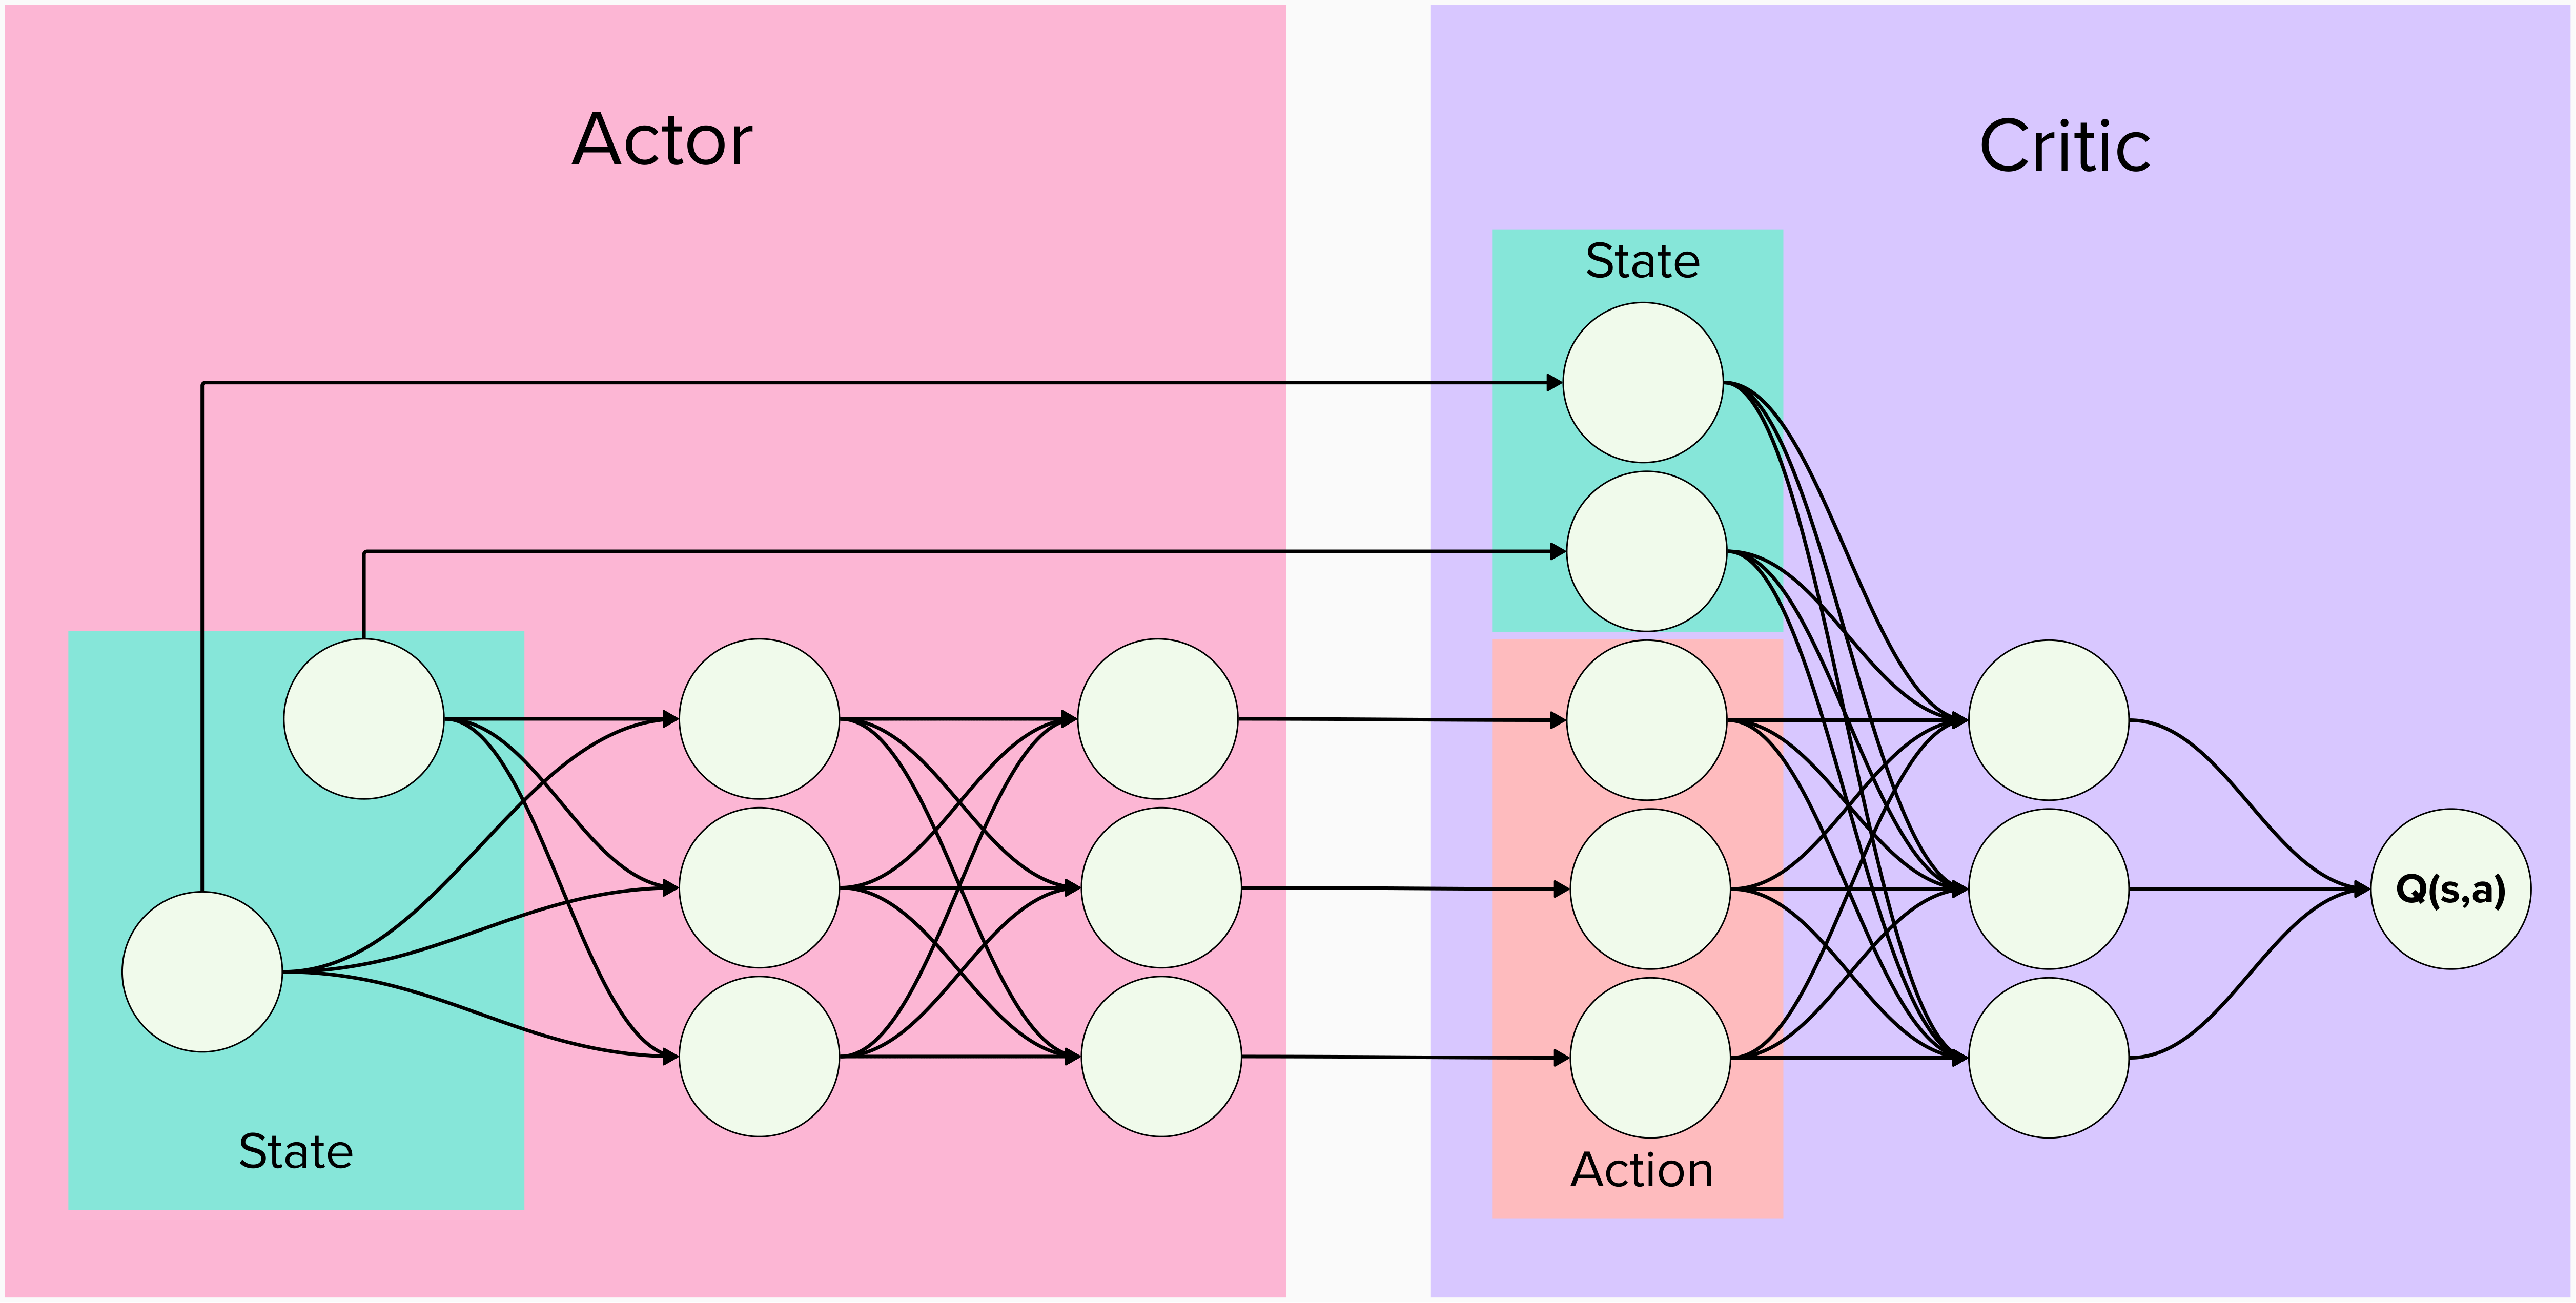
\includegraphics[width=0.65\textwidth]{2Grundlagen/35Actor_Critick.png}
\caption{Illustration des Actors und Critics im DDPG-Algorithmus.}
\label{fig:actor_critick}
\end{figure}

\paragraph{Die Rolle des Actors}
Der Actor \ref{fig:actor_critick} hat die Aufgabe, eine optimale Policy \(\mu(s)\) zu erlernen, die für jeden gegebenen Zustand \(s\) eine Aktion \(a\) ausgibt, mit dem Ziel, den erwarteten Reward zu maximieren \cite{SuttonBarto2018}. Diese Policy-Funktion wird in einem kontinuierlichen Aktionsraum direkt modelliert, wobei jede Aktion ein kontinuierlicher Wert ist. Der Actor ist daher das Entscheidungselement innerhalb der Architektur \cite{SuttonBarto2018}.


\paragraph{Die Funktion des Critics}
\label{sec: Rolle des Critics}
Der Critic \ref{fig:actor_critick} hingegen bewertet die Aktionen, die vom Actor vorgeschlagen werden wie in Abbildung \ref{fig:get_q_value_critic} gezeigt. Er nimmt den aktuellen Zustand und die vom Actor vorgeschlagene Aktion auf und schätzt den Q-Wert \( Q(s,a) \). Diese Schätzung repräsentiert den erwarteten zukünftigen Reward, der aus der Ausführung der Aktion \( a \) im Zustand \( s \) resultiert, noch bevor die eigentliche Simulation in der Umgebung gestartet wird \cite{SuttonBarto2018}. Somit versucht der Critic, die Qualität einer Aktion im Kontext des aktuellen Zustands zu bewerten und liefert dem Actor Feedback, das zur Optimierung der Policy verwendet wird.

\paragraph{Die Actor-Critic-Interaktion}
In Abbildung \ref{fig:actor_critick} ist die Interaktion zwischen dem Actor und dem Critic illustriert. Der Actor generiert Aktionen basierend auf der aktuellen Policy, und der Critic bewertet diese Aktionen, indem er den Q-Wert zur Verfügung stellt. Diese Interaktion ermöglicht es dem DDPG-Algorithmus, sowohl die optimale Policy als auch die Wertfunktion effektiv zu lernen \cite{SuttonBarto2018}.


\paragraph{Aktualisierung des Critics im DDPG}

Die Aktualisierung des Critics im Deep Deterministic Policy Gradient Algorithmus ist ein entscheidender Schritt für das effektive Lernen von handlungsorientierten Strategien in kontinuierlichen Aktionsräumen. Die grundlegende Idee des DDPG ist es, die Stärken von Q-Learning \ref{eq: update q learning} und Policy Gradient Methoden \ref{eq:policy_gradient} zu kombinieren, um die Effizienz des Lernprozesses in solchen Umgebungen zu verbessern \cite{Lillicrap2016DDPG}.


\paragraph{Update-Prinzip des Critics}
\begin{figure}[htbp]
\centering
  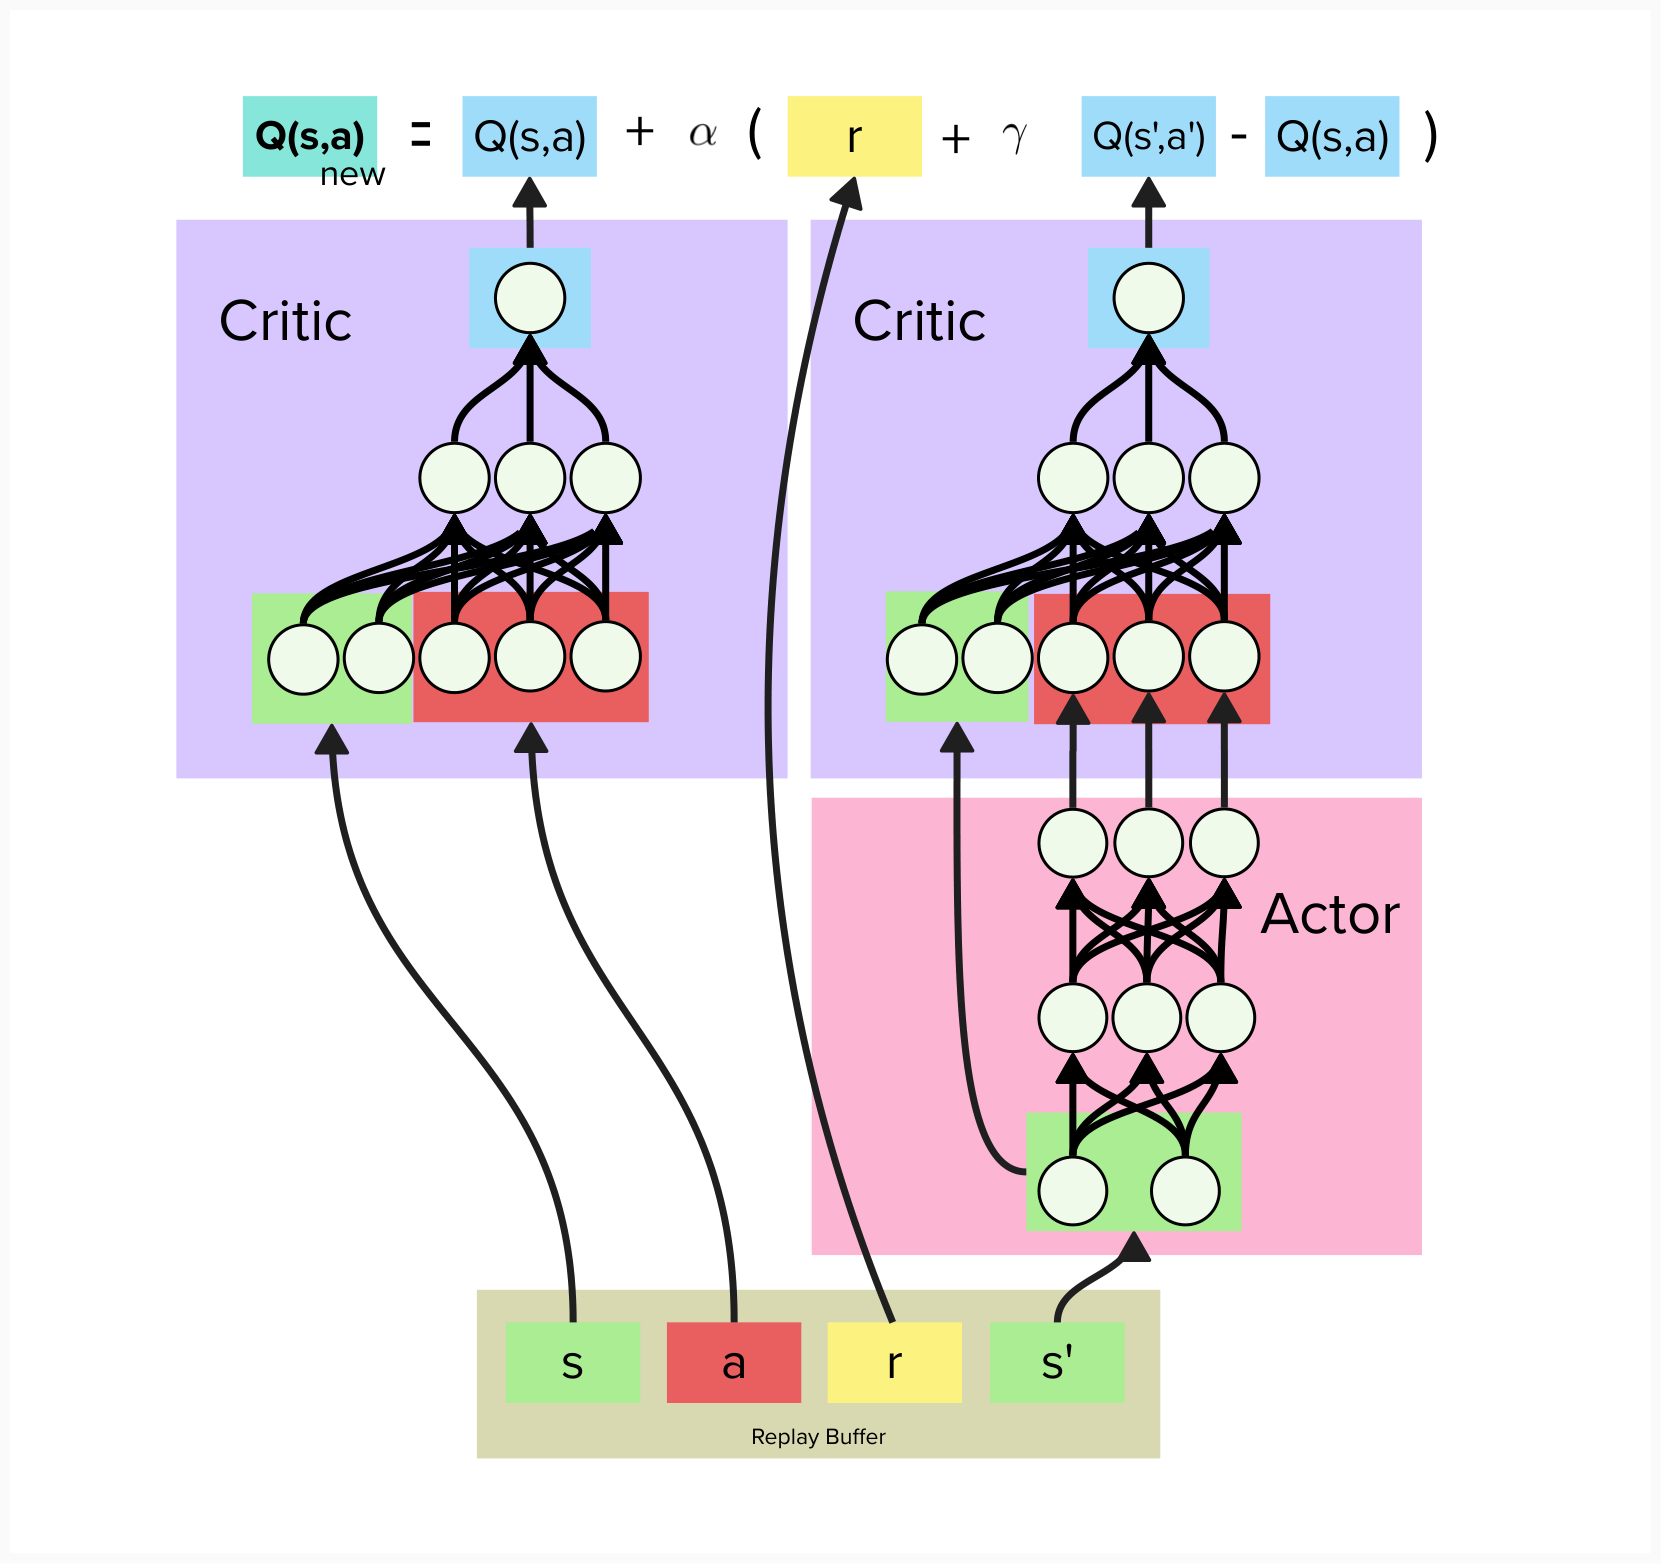
\includegraphics[width=0.70\textwidth, trim=10px 10px 10px 10px, clip]{2Grundlagen/35Q_value_Critick.png}
  \captionof{figure}[Berechnung des Q-Werts]{Berechnung des Q-Werts durch den Critic (Quelle: \cite{wei2020ddpg}).}
  \label{fig:get_q_value_critic}
\end{figure}
Der Critic bewertet die Politik des Actors, indem er die Q-Werte für die vom Actor vorgeschlagenen Aktionen schätzt. Diese Q-Werte repräsentieren das erwartete zukünftige Reward für den Zustand-Aktions-Paar (\(s, a\)). Der Critic wird aktualisiert, indem der Temporal Difference (TD) Error minimiert wird \ref{eq:Ketten Regel},  der die Differenz zwischen den geschätzten Q-Werten und den tatsächlichen Rewards aus der Umgebung widerspiegelt \cite{Wu2018AggregatedMultiDDPG}. Die Update-Regel für den Critic ist eine Variante der Bellman-Gleichung \ref{eq: Bellman } , die im DQN verwendet wird \ref{eq: update q learning}, und kann formal durch die folgende Gleichung ausgedrückt werden:



\begin{equation}
		Q(s,a) \leftarrow Q(s,a) + \alpha \cdot (r + \gamma \cdot Q(s',\mu(s') - Q(s,a)))
		\label{eq:critick update}
\end{equation}

Hierbei ist \( \alpha \) die Lernrate, \( r \) der sofortige Reward, \( \gamma \) der Diskontierungsfaktor für zukünftige Rewards, und \( \mu(s') \) die Policy des Actors, die den nächsten Zustand \( s' \) auf die nächste Aktion abbildet, wie in Abbildung \ref{fig:get_q_value_critic} gezeigt.



Der TD Error für das Training des Critics kann dann als die Differenz zwischen dem geschätzten Q-Wert und dem Target-Q-Wert definiert werden:
\[ TD_{error} = Q_{target}(s_t, a_t) - Q(s_t, a_t) \]
Diese Diskrepanz wird quadriert \ref{eq:cost_function}, um als Loss-Funktion zu fungieren, die dann minimiert wird , um das Lernen zu verbessern \ref{eq:partial_derivative} \cite{SuttonBarto2018}.

\begin{figure}[htbp]
\centering
  \centering
  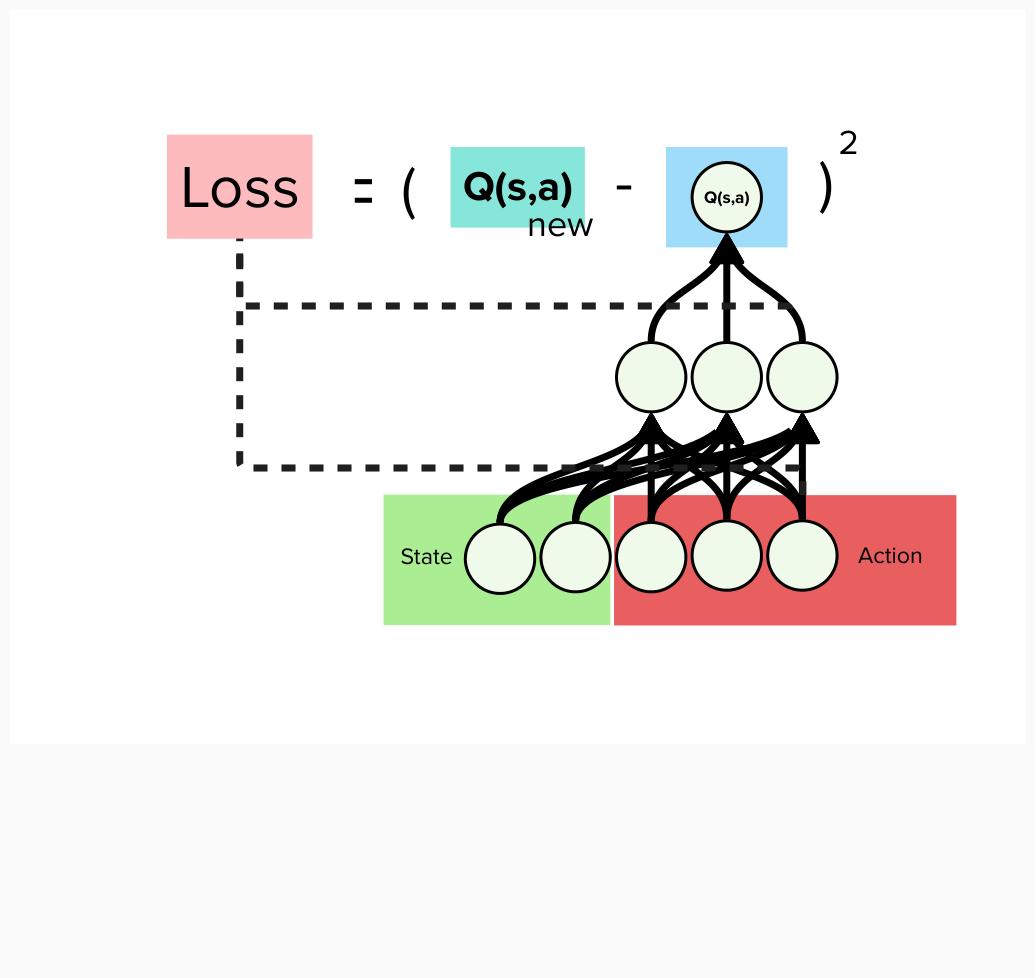
\includegraphics[width=0.45\textwidth, trim=10px 10px 10px 10px, clip]{2Grundlagen/35Q_value_Critick_update.png}
  \captionof{figure}[Aktualisierung des Q-Werts]{Aktualisierung des Q-Werts im Critic-Netzwerk.}
  \label{fig:update_q_value}
\end{figure}



\paragraph{Gradient Descent und Kettenregel}
Um die Gewichte des Critics zu aktualisieren, wird der Gradient Descent angewendet, wobei der Gradient der Loss-Funktion in Bezug auf die Gewichte berechnet \ref{eq: gradient matrix} und die Gewichte entsprechend angepasst werden \cite{aggarwal_neural_networks_2018}.




\paragraph{Bedeutung der Kritik}
Die Funktion des Critics ist es nicht nur, die Aktionen des Actors zu bewerten, sondern auch, eine Lernsignal für den Actor zu generieren. Dies geschieht durch die Rückkopplung des TD Errors an den Actor, wodurch dieser informiert wird, welche Aktionen zu einer Verbesserung oder Verschlechterung des erwarteten Rewards führen. Der Actor nutzt diese Information, um seine Policy in Richtung von Aktionen zu steuern, die zu einem höheren Reward führen \cite{Luck2019ImprovedExploration}.


\paragraph{Optimierung des Actor-Netzwerks im DDPG}

In Anlehnung an die zuvor dargestellte Aktualisierung des Critics ist das Ziel des Actor-Updates, eine Policy-Funktion zu erlernen, die Aktionen ausgibt, um den erwarteten Reward zu maximieren. Dieser Lernprozess basiert auf der Rückkopplung durch den Critic, der bereits präzise Q-Werte liefert. Die Aktualisierung erfolgt durch Anwendung eines Gradienten-Ascent-Verfahrens, welches auf die Maximierung der Q-Werte ausgerichtet ist \cite{Lillicrap2016DDPG, Wu2018AggregatedMultiDDPG}.


Die mathematische Darstellung des Updates wird durch die Gleichung ausgedrückt, die die Ableitung des Losses in Bezug auf die Parameter \(\theta_\mu\) des Actor-Netzwerks darstellt:
\begin{equation}
\nabla_{\theta_\mu} \text{LOSS}_{Actor} = -\mathbb{E}_{s \sim \mathcal{D}} \left[ \nabla_a Q(s, a)|_{a=\mu(s)} \nabla_{\theta_\mu} \mu(s) \right]
		\label{eq:actor update}
\end{equation}


\begin{figure}[htbp]
\centering
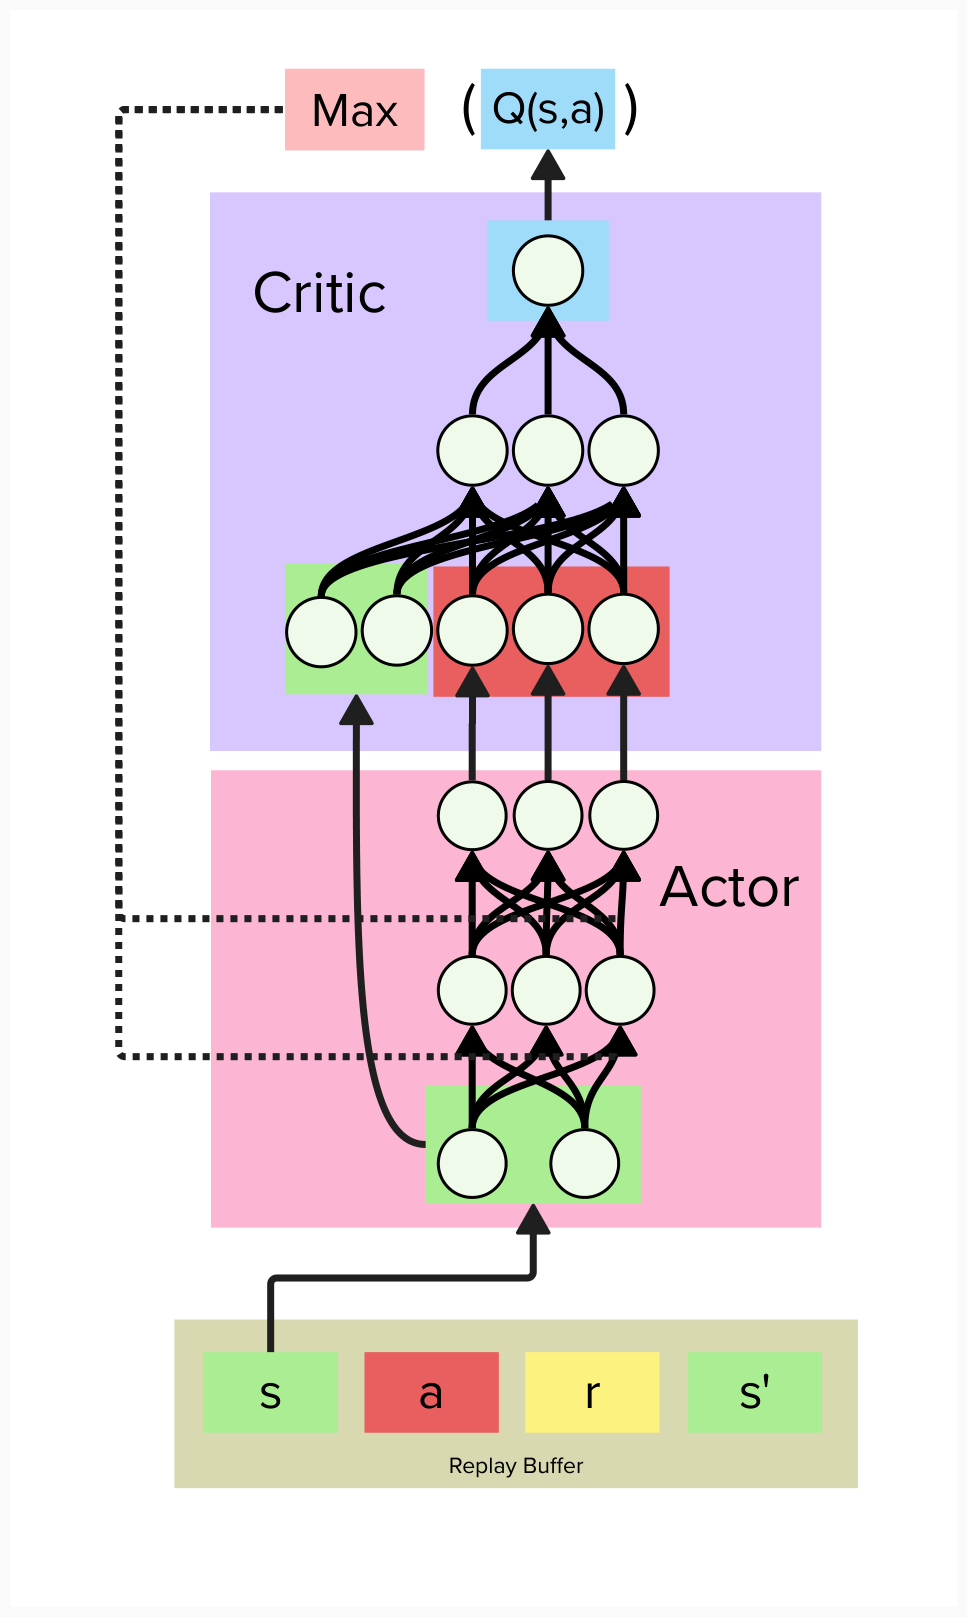
\includegraphics[width=0.45\textwidth, trim=10px 10px 10px 10px, clip]{2Grundlagen/35_update_actor.png}
\captionof{figure}[Aktualisierung des Actors]{Gradienten-Ascent für die Aktualisierung des Actors, um die Q-Werte zu maximieren. Der Actor nutzt die vom Critic berechneten Q-Werte, um die Policy-Funktion zu optimieren und den erwarteten Reward zu maximieren.}
\label{fig:update_actor}
\end{figure}

\paragraph{Der Update-Mechanismus des Actors}
Wie in Abbildung \ref{fig:update_actor} dargestellt, zielt das Update des Actors darauf ab, eine Policy-Funktion zu erlernen, die Aktionen so ausgibt, dass der erwartete Reward maximiert wird.Der Actor wählt Aktionen anhand der aktuellen Policy aus, die anschließend in der Umgebung ausgeführt werden, was zur Transition von Zustand \(s\) zu Zustand \(s'\) und zur Vergabe eines Rewards führt. Wie in \cite{Lillicrap2016DDPG} beschrieben, wird der Actor durch die Anwendung der Kettenregel \ref{eq:Ketten Regel} auf den erwarteten Return aus der Startverteilung aktualisiert, was eine direkte Anpassung der Actor-Parameter ermöglicht. Die Verlustfunktion des Actors wird durch die negativen Gradienten der Q-Werte in Bezug auf die Aktionen, berechnet an der Stelle der durch die Policy vorgeschlagenen Aktionen, definiert. Diese wird dann genutzt, um die Parameter der Actor-Policy in Richtung eines höheren erwarteten Rewards zu verschieben \cite{Lillicrap2016DDPG}.


\paragraph{Die Bedeutung der Aktualisierung des Actors}
Die Aktualisierung des Actors ist ein kritischer Schritt im Lernprozess, da sie das Trainingssignal für den Actor aus den Bewertungen des Critics ableitet. Diese Interaktion ermöglicht es dem Actor, seine Policy zu verbessern und optimale Aktionen im Kontext der gegebenen Umgebung auszuwählen \cite{Luck2019ImprovedExploration}. Die kontinuierliche Verbesserung der Policy durch den Actor führt zu einer verbesserten Entscheidungsfindung und letztlich zu einem höheren kumulativen Reward.

DDPG nutzt die Experience Replay-Technik, die zuerst in DQN eingeführt wurde \ref{eq:replay buffer}, um die Korrelation zwischen aufeinanderfolgenden Lernschritten zu reduzieren. Dies erhöht die Datenvarianz und hilft, eine stabilere und effektivere Lernumgebung zu schaffen, wie in \cite{Wu2018AggregatedMultiDDPG} beschrieben. 


\paragraph{Exploration und Exploitation im DDPG}

Der DDPG-Algorithmus erweitert die traditionelle \(\epsilon\)-greedy Strategie \ref{eq:epsilon_greedy} um eine raffinierte Explorationstaktik, bei der ein kontrolliertes Rauschen auf die Auswahl kontinuierlicher Aktionen angewendet wird. Dieses adaptive Rauschen, wie  Simulated-Annealing-Prozess \ref{sec:Simulated Annealing}, wird schrittweise verringert und ermöglicht so eine effektive Exploration des Aktionsraums. Durch diese graduelle Reduktion, verringert der Algorithmus die anfängliche Abhängigkeit von der Rauschintensität und fördert die Entdeckung optimaler Handlungsstrategien.


\paragraph{Integration von Experience Replay}

Neben dieser adaptiven Explorationsmethode implementiert DDPG auch die Erfahrungswiedergabe (siehe Gleichung \ref{eq:replay buffer}), ein Ansatz, der zuerst in DQN zum Einsatz kam. Diese Technik ist entscheidend, um die Abhängigkeiten zwischen aufeinanderfolgenden Stichproben zu beseitigen und sie als unabhängig und identisch verteilt zu behandeln, was die Stabilität des Lernprozesses deutlich erhöht \cite{Wu2018AggregatedMultiDDPG}. Die Anpassung des Actor-Netzwerks, das die zugrundeliegende Policy repräsentiert, folgt konsequent den Prinzipien der Kettenregel und der Rückpropagation, um eine konvergente Annäherung an die optimale Policy zu gewährleisten, die wiederum die Gesamteffizienz des Algorithmus steigert \cite{Wu2018AggregatedMultiDDPG}.

\begin{figure}[htbp]
\centering
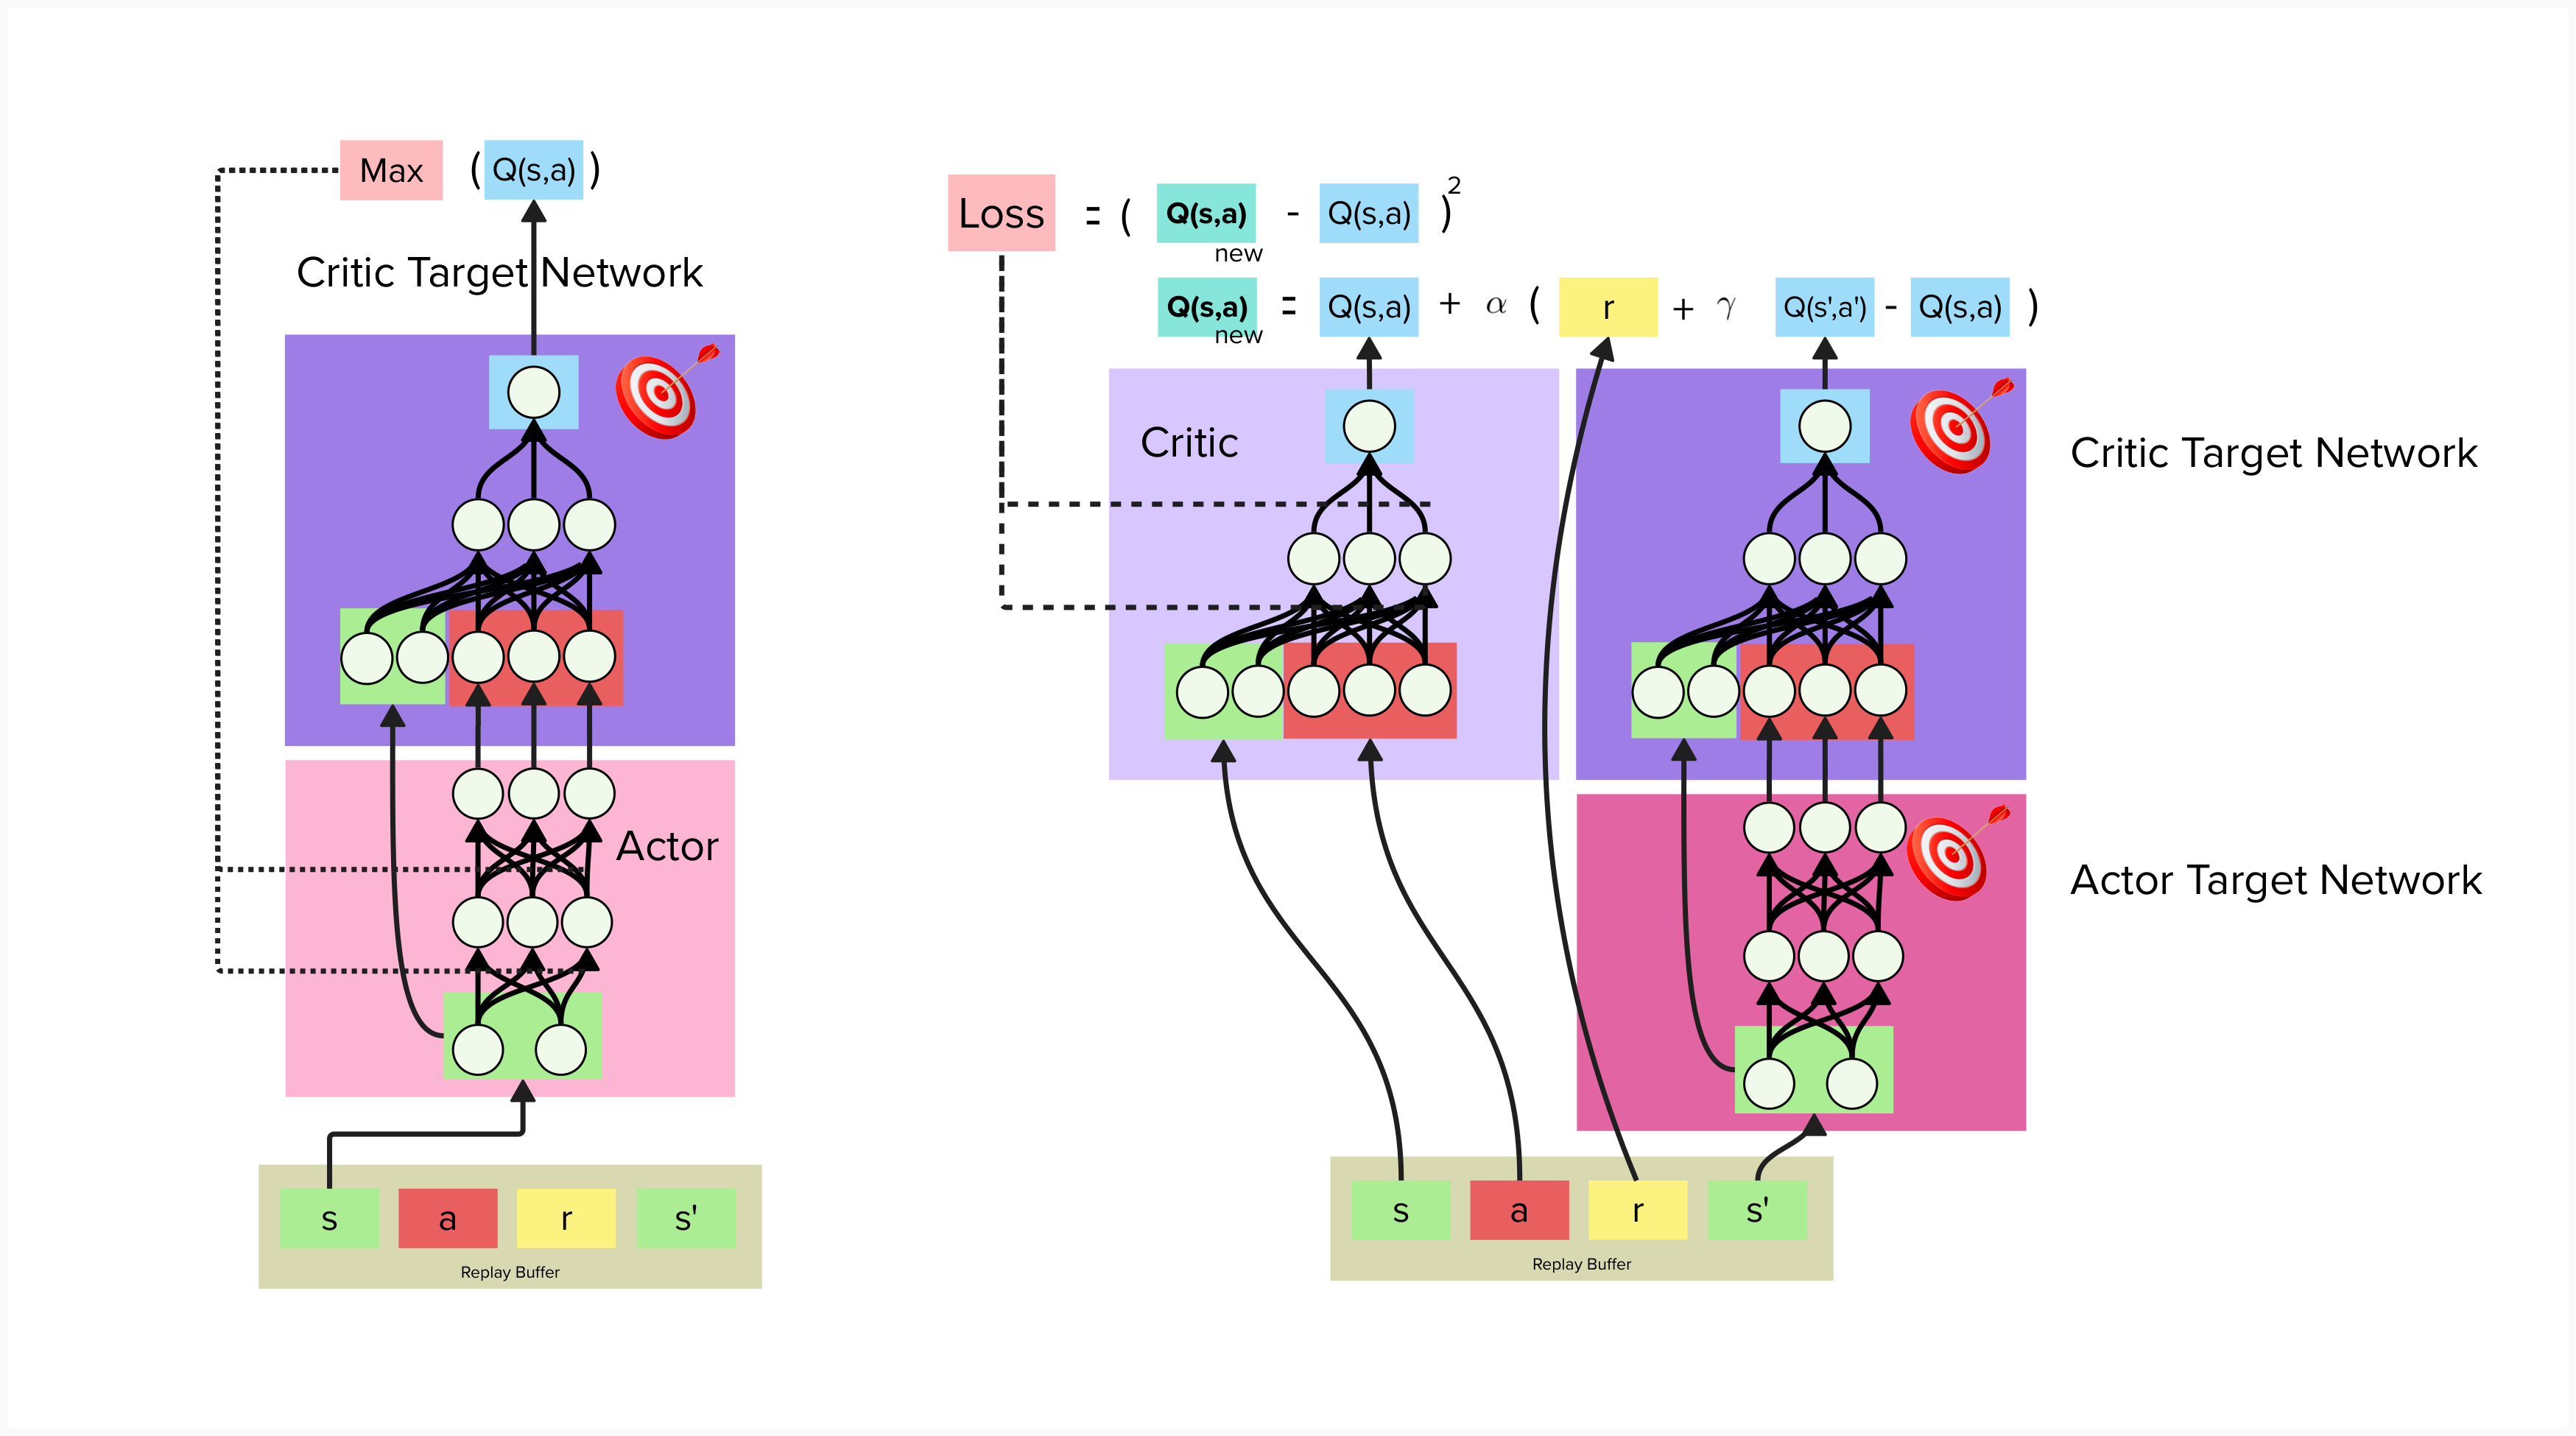
\includegraphics[width=0.99\textwidth, trim=10px 10px 10px 10px, clip]{2Grundlagen/35critick_actor_target.png}
\caption{Interaktion zwischen Actor, Critic und den Target Networks im DDPG-Algorithmus.}
\label{fig:actor_critic_diagram}
\end{figure}

\paragraph{Die Rolle der Target Networks im DDPG}
Im DDPG-Algorithmus werden Target Networks eingesetzt, um die Stabilität während des Trainings zu erhöhen. Diese Netzwerke sind Kopien des Critic und des Actor, die mit einem geringeren Update-Faktor \( \tau \) aktualisiert werden. Durch diese verzögerte Aktualisierung dienen die Target Networks als langsam veränderliche Zielwerte für die Updates des Critic und des Actor. Dies trägt dazu bei, die Korrelation zwischen den Schätzungen von \( Q(s,a) \) und \( Q(s',a') \) zu verringern und verhindert damit, dass der Lernalgorithmus durch schnelle Änderungen der bewerteten Policies instabil wird \cite{Wu2018AggregatedMultiDDPG}. Während des Trainingsprozesses bleibt das Target Network fest, das heißt, seine Gewichte werden nicht bei jedem Schritt aktualisiert, sondern in regelmäßigen Abständen, um die Stabilität der Zielwerte zu gewährleisten. Dies bedeutet, dass das Target Network als Ankerpunkt für den Actor und den Critic fungiert und ihnen eine konsistente Richtung für die Aktualisierung gibt. Insbesondere beim Update des Critics wird der TD-Fehler gegen die stabilen Zielwerte des Target Networks berechnet, was die Varianz der Updates reduziert und die Konvergenz des Netzwerks fördert. Beim Aktualisieren des Actors hingegen wird die Policy basierend auf einer Rückkopplung optimiert, die von den stabilen Q-Werten des Critic Target Networks abgeleitet ist. Die Verwendung von Target Networks im DDPG ist analog zum Einsatz des Experience Replay: Beide Techniken zielen darauf ab, die Korrelationen zwischen aufeinanderfolgenden Lernschritten zu reduzieren und die Datenvarianz zu erhöhen. Sie helfen dabei, eine stabilere und effektivere Lernumgebung zu schaffen, wie in der Forschung von \cite{Luck2019ImprovedExploration} und \cite{Wu2018AggregatedMultiDDPG} beschrieben.
 

\paragraph{Überleitung zu praktischen Anwendungen}
Nachdem die Grundlagenkapitel die Schlüsseltechniken des maschinellen Lernens, wie die Vorwärts- und Rückwärtspropagation, die Berechnung von Gradienten sowie verschiedene Netzwerkarchitekturen, eingeführt haben, steht nun die Anwendung dieser Methoden auf reale Probleme im Fokus. Im nächsten Kapitel werden wir die Leistungsfähigkeit von RL-Techniken an einem praktischen Beispiel demonstrieren: der Optimierung von PID-Reglern für die Steuerung von DC-DC-Wandlern. Unser Ziel ist es, einen Actor zu trainieren, der in der Lage ist, die PID-Koeffizienten präzise anzupassen, um auf verschiedene Degradationsstufen des Wandlers zu reagieren und somit seine Effizienz signifikant zu steigern. Diese Anwendung repräsentiert eine Brücke zwischen theoretischen Konzepten und realen ingenieurtechnischen Herausforderungen und zeigt, wie fortgeschrittene Algorithmen des maschinellen Lernens zur Lösung komplexer Steuerungsprobleme beitragen können.





%Hyperparameter und Regularisierung
  %Learning Rate
  %Batch Size
  %Overfitting und Regularisierung
  %Normalization (Batch, Layer)
  

%Evaluationsmetriken
  %Klassifikation: Genauigkeit, F1-Score etc.
  %Reinforcement Learning: Reward-Metriken

%Reinforcement Learning
  %Grundlagen und Prinzipien
  %Markov-Entscheidungsprozesse (MDPs)
  %Belohnungssystem
  %Exploration vs Exploitation
  %Policy vs. Value-based Methods

%Regularisierung in RL
  %Entropie-Regularisierung etc.

%Fortgeschrittene Themen in Deep Learning
  %Deep Q-Learning
  %Actor-Critic-Methoden
  %DDPG (Deep Deterministic Policy Gradients)


